\section{Affiliated Values I: Equilibrium Bidding}\label{sec:14-mw-eq}

The private-values theory of \cref{sec:14-spa,sec:14-fpa,sec:14-ret,sec:14-optimal} rests on two
assumptions. Each bidder knows the value of the object to itself, and values are statistically independent.
Many of the auctions that motivate the theory violate both. An oil company bidding for a drilling lease does
not know how much oil lies under the tract, and its geologists' estimate is correlated with the estimates of
its rivals. This section and the next study the model of \citet{MilgromWeber1982}, which drops both
assumptions at once and still delivers sharp predictions. Their model became the standard framework for
auctions with interdependent values, and we treat the paper as a deep dive.

This section sets out the questions, the model and the properties of affiliation, and then derives the
symmetric equilibria of the second-price, English and first-price auctions. It also covers bidders with
inferior information, including the one-informed-bidder model that \citet{HendricksPorter1988} take to
offshore oil data. \Cref{sec:14-mw-rank} uses these equilibria to rank the formats by expected revenue,
studies the seller's disclosure of information, reserve prices, entry fees and risk aversion, and assesses
the paper. We keep the book's conventions from \cref{sec:14-info}. Bidder $i$'s signal is $S_i$ (Milgrom and
Weber write $X_i$), other value-relevant variables are $\bm A=(A_1,\dots,A_m)$ (their $S$), and the seller's
information is $S_0$ (their $X_0$).

\subsection{The question and the setting}\label{sec:14-mw-question}

\citet[pp.~1089--1090]{MilgromWeber1982} open with two sets of questions. The first concerns design. Why do
the English, Dutch, first-price and second-price auctions coexist, and which one should a seller use in a
given circumstance? The second concerns the link with competitive theory. Do auction prices resemble
competitive prices, and do they approach them when there are many bidders? When bidders hold different
information about the intrinsic qualities of the object, do prices aggregate that information, as they do in
rational expectations models of markets? Answering either set requires a model in which one bidder's
information matters for the value that others place on the object.

The benchmark at the time was the independent private values model, which
\citet[pp.~1090--1093]{MilgromWeber1982} summarize in seven conclusions. All of them appear earlier in this
chapter.
\begin{enumerate}[label=(\arabic*)]
  \item The Dutch and first-price auctions are strategically equivalent (\cref{prop:14-dutch-fpa}).
  \item With private values, the second-price and English auctions are equivalent in a weaker sense. Each has
  a dominant strategy, bidding (or staying in up to) one's value, and the two lead to the same outcome
  (\cref{sec:14-spa}).
  \item The English and second-price auctions allocate the object to the bidder who values it most, so their
  outcomes are Pareto optimal. In symmetric models the Dutch and first-price auctions do so as well
  (\cref{sec:14-fpa}).
  \item All four formats yield the same expected revenue (\cref{prop:14-ret}).
  \item The self-selection approach explains this. Any mechanism that gives the object to the highest
  valuation and leaves the lowest type a zero payment yields the expected second-highest valuation
  (\cref{sec:14-ret}).
  \item For many common distributions, including the normal, exponential and uniform, the standard formats
  with a suitable reserve price or entry fee are optimal mechanisms (\cref{sec:14-optimal}).
  \item When bidders are risk averse, the seller strictly prefers the Dutch or first-price auction to the
  English or second-price auction (\cref{prop:14-risk-fpa}).
\end{enumerate}
For the design question this benchmark gives little guidance. Its main prediction is that the four common
formats raise the same expected price \citep[p.~1095]{MilgromWeber1982}.

Mineral rights are the leading example of a different environment \citep[Section~2.2]{MilgromWeber1982}.
To a first approximation the rights are worth the same to every bidder, and bidders differ only in their
estimates of this common value. \Cref{sec:14-winners-curse} described the resulting winner's curse and the
two results of the mineral rights literature that foreshadow the general theory. Prices can aggregate
dispersed information (\cref{rem:14-aggregation}), and a bidder's profit depends more on the privacy of its
information than on its accuracy (\cref{rem:14-privacy}). We prove a version of the second result in
\cref{sec:14-mw-inferior}.

The sale of a painting (\cref{sec:14-info-model}) shows why a general model is needed. Resale, prestige and
doubts about authenticity break private values, and related information breaks independence. The common
value model allows for statistical dependence but leaves no room for differences in tastes. Milgrom and Weber
build a model that contains both the private values and common value models and the intermediate cases
between them. Despite its generality, the model yields testable predictions
\citep[pp.~1095--1097]{MilgromWeber1982}.
\begin{enumerate}[label=(\roman*)]
  \item The Dutch and first-price auctions remain strategically equivalent.
  \item When bidders are uncertain about their own values, the English auction generates higher expected
  prices than the second-price auction. Bidders learn from the prices at which rivals drop out, which
  weakens the winner's curse and makes them bid more aggressively.
  \item When value estimates are positively dependent, the second-price auction generates higher expected
  prices than the first-price auction. The formats are ranked English, then second price, then Dutch and
  first price. Milgrom and Weber suggest that this ranking may explain an observation by Cassady. In his
  words, ``an estimated 75 per cent, or even more, of all auctions in the world are conducted on an
  ascending-bid basis'' \citep[p.~66, quoted in Milgrom and Weber 1982, p.~1095]{Cassady1967}.
  \item A seller with private information can commit to concealing it, reporting it fully, censoring it,
  summarizing it or adding noise to it. In the first-price, second-price and English auctions, reporting it
  fully maximizes the expected price.
  \item Holding fixed the set of bidders who participate, it pays to raise entry fees and lower reserve
  prices.
  \item With risk-averse bidders, the first-price and second-price auctions cannot be ranked in general. With
  constant absolute risk aversion, the English auction still beats the second-price auction and full
  disclosure remains optimal in both.
\end{enumerate}
The rest of this section and the next derive each prediction.

\subsection{The model}\label{sec:14-mw-model}

We work with the general symmetric model of \cref{sec:14-info-model} and maintain \cref{ass:14-mw}
throughout this section and the next. There are $n\ge 2$ bidders and one indivisible object. Bidder $i$
observes a real-valued signal $S_i$ with realization $s_i$, which we also call its \emph{value estimate}. The
vector $\bm A=(A_1,\dots,A_m)$ collects the other variables that affect the value of the object, such as an
expert appraisal or the tastes of future buyers. The value to bidder $i$ is $V_i=u(\bm A,S_i,\bm S_{-i})$,
which may depend on variables that bidder $i$ does not observe. Private values are the case $m=0$ and
$V_i=S_i$, and the pure common value model is the case $m=1$ and $V_i=A_1$. Bidders are risk neutral until
\cref{sec:14-mw-risk}. A bidder who wins and pays $b$ receives $V_i-b$, and losers receive zero.

By symmetry we can study bidder 1. Let $Y_1\ge Y_2\ge\dots\ge Y_{n-1}$ denote the order statistics of the
rivals' signals $S_2,\dots,S_n$, largest first. Because $u$ is symmetric in the rivals' signals, bidder 1's
value depends on them only through their order statistics:
\begin{equation}\label{eq:14-mw-V1}
  V_1=u(\bm A,S_1,Y_1,\dots,Y_{n-1}).
\end{equation}
The joint density of $(\bm A,S_1,Y_1,\dots,Y_{n-1})$ is \eqref{eq:14-joint-orderstat}, which is
$(n-1)!$ times the density $f$ restricted to ordered vectors of rival signals.

The function that drives all equilibria is the expected value of the object to bidder 1 when its signal is
$s$ and the highest rival signal is $y$:
\begin{equation}\label{eq:14-mw-v}
  v(s,y)=\E\left[V_1\mid S_1=s,\,Y_1=y\right].
\end{equation}
We write $F_{Y_1}(\cdot\mid s)$ and $f_{Y_1}(\cdot\mid s)$ for the conditional distribution function and
density of $Y_1$ given $S_1=s$, and $[\underline s,\bar s]$ for the support of each signal. Milgrom and Weber
add a \emph{nondegeneracy} assumption, namely that $\E[V_1\mid S_1=s,Y_1=y_1,\dots,Y_{n-1}=y_{n-1}]$ is
strictly increasing in $s$. It shortens proofs, and all results hold without it
\citep[p.~1100]{MilgromWeber1982}. A strategy for bidder $i$ is a function $\beta_i:[\underline s,\bar s]\to\R_+$
from signals to bids. We study symmetric equilibria in which every bidder uses the same strictly increasing
$\beta$.

\subsection{Properties of affiliation}\label{sec:14-mw-affil}

Affiliation was defined in \cref{def:14-affiliation}, and \cref{prop:14-affil-char} gave its
characterization for smooth densities (Milgrom and Weber's Theorem 1). \Cref{prop:14-affil-props} listed the
four further properties that the equilibrium analysis uses (their Theorems 2 to 5), and
\cref{sec:14-affiliation} proved part (iv), which concerns order statistics. We now prove the other three
parts, or sketch the proofs, in the generality that we need.

\begin{proof}[Proof of \cref{prop:14-affil-props}, parts (i) to (iii)]
\emph{Part (i).} We prove the case of strictly increasing, differentiable $g_j$, which covers our applications.
Let $\bm W=(g_1(Z_1),\dots,g_k(Z_k))$ and $\bm g^{-1}(\bm w)=(g_1^{-1}(w_1),\dots,g_k^{-1}(w_k))$. The
change-of-variables formula gives the density of $\bm W$:
\begin{equation*}
  f_{\bm W}(\bm w)=f\left(\bm g^{-1}(\bm w)\right)J(\bm w),\qquad
  J(\bm w)=\prod_{j=1}^k\frac{d g_j^{-1}(w_j)}{dw_j}.
\end{equation*}
Each $g_j^{-1}$ is increasing and acts on one coordinate, so
$\bm g^{-1}(\bm w\vee\bm w')=\bm g^{-1}(\bm w)\vee\bm g^{-1}(\bm w')$, and similarly for $\wedge$. The
affiliation of $f$ then gives
$f(\bm g^{-1}(\bm w\vee\bm w'))f(\bm g^{-1}(\bm w\wedge\bm w'))\ge f(\bm g^{-1}(\bm w))f(\bm g^{-1}(\bm w'))$.
For the Jacobian, the pair $\{\max\{w_j,w_j'\},\min\{w_j,w_j'\}\}$ equals the pair $\{w_j,w_j'\}$ in every
coordinate, so $J(\bm w\vee\bm w')J(\bm w\wedge\bm w')=J(\bm w)J(\bm w')$. Multiplying the two relations
proves the claim. If all $g_j$ are decreasing, then $\bm g^{-1}(\bm w\vee\bm w')=\bm g^{-1}(\bm w)\wedge
\bm g^{-1}(\bm w')$, and the argument goes through because \eqref{eq:14-affil-ineq} is symmetric in the roles
of $\vee$ and $\wedge$. Weakly monotone transformations can create atoms, and they require the general
definition of affiliation in Milgrom and Weber's Appendix.

\emph{Parts (ii) and (iii).} Milgrom and Weber derive both from the characterization of affiliation as
conditional association in \cref{prop:14-association}(b). For densities, \citet{KarlinRinott1980} prove
directly that integrating out a variable preserves \eqref{eq:14-affil-ineq}, which is part (ii). Part (iii)
follows from the conditional association inequality applied to $g=H$ and to indicators of increasing sets
\citep[see also][]{Whitt1982}. We prove (iii) in the bivariate case that we use most often. Let $(Z_1,Z_2)$
have an affiliated density, let $H$ be nondecreasing, and consider $\E[H(Z_2)\mid Z_1=z,\,Z_2\le x]$.
Conditional on $Z_1=z$ and $Z_2\le x$, $Z_2$ has density $\frac{f(y\mid z)}{F(x\mid z)}$ on $y\le x$. For
$z'>z$ the ratio of the densities under $z'$ and $z$ is $\frac{f(y\mid z')F(x\mid z)}{f(y\mid z)F(x\mid z')}$,
which is nondecreasing in $y$ by the monotone likelihood ratio property (\cref{prop:14-affil-mlrp}). A
likelihood ratio ordering implies first-order stochastic dominance, so the conditional mean of the
nondecreasing function $H$ rises with $z$. For $x'>x$, the ratio of the densities truncated at $x'$ and at
$x$ equals the constant $\frac{F(x\mid z)}{F(x'\mid z)}$ on $y\le x$ and is infinite on $(x,x']$. It is
nondecreasing in $y$, so the mean rises with $x$ as well.
\end{proof}

Two consequences are used repeatedly.

\begin{corollary}\label{cor:14-mw-v}
Under \cref{ass:14-mw}, $(S_1,Y_1)$ are affiliated, and $v(s,y)$ is nondecreasing in both arguments. Under
nondegeneracy, $v$ is strictly increasing in $s$.
\end{corollary}

\begin{proof}
Affiliation of $(S_1,Y_1)$ follows from parts (iv) and (ii) of \cref{prop:14-affil-props}. Let
\begin{equation*}
  \bar v(s,y_1,\dots,y_{n-1})=\E\left[V_1\mid S_1=s,\,Y_1=y_1,\dots,Y_{n-1}=y_{n-1}\right].
\end{equation*}
By \eqref{eq:14-mw-V1}, $\bar v$ is the conditional mean of the nondecreasing function $u$ of the affiliated
vector of \cref{prop:14-affil-props}(iv), so it is nondecreasing by part (iii). The law of iterated
expectations gives
\begin{equation*}
  v(s,y)=\E\left[\bar v(S_1,Y_1,\dots,Y_{n-1})\mid S_1=s,\,Y_1=y\right],
\end{equation*}
which is nondecreasing by part (iii) again. If $\bar v$ is strictly increasing in $s$ and $s'>s$, then
\begin{align*}
  v(s',y)&=\E[\bar v(s',y,Y_2,\dots,Y_{n-1})\mid S_1=s',Y_1=y]\\
  &>\E[\bar v(s,y,Y_2,\dots,Y_{n-1})\mid S_1=s',Y_1=y]\\
  &\ge\E[\bar v(s,y,Y_2,\dots,Y_{n-1})\mid S_1=s,Y_1=y]=v(s,y).\qedhere
\end{align*}
\end{proof}

\begin{lemma}[{\citealp[Lemma~1]{MilgromWeber1982}}]\label{lem:14-mw-lemma1}
Under \cref{ass:14-mw}, $\frac{F_{Y_1}(y\mid z)}{f_{Y_1}(y\mid z)}$ is nonincreasing in $z$.
\end{lemma}

\begin{proof}
Let $g(z,y)$ be the joint density of $(S_1,Y_1)$, which is affiliated by \cref{cor:14-mw-v}. Take
$\alpha\le y$ and $z'\le z$, and apply \eqref{eq:14-affil-ineq} to the points $(z,\alpha)$ and $(z',y)$.
Their componentwise maximum is $(z,y)$ and their minimum is $(z',\alpha)$, so
\begin{equation*}
  g(z,y)\,g(z',\alpha)\ge g(z,\alpha)\,g(z',y).
\end{equation*}
Dividing both sides by the marginal densities of $S_1$ at $z$ and $z'$ turns joint densities into
conditional densities:
\begin{equation*}
  f_{Y_1}(y\mid z)\,f_{Y_1}(\alpha\mid z')\ge f_{Y_1}(\alpha\mid z)\,f_{Y_1}(y\mid z').
\end{equation*}
Rearranging gives
$\frac{f_{Y_1}(\alpha\mid z)}{f_{Y_1}(y\mid z)}\le\frac{f_{Y_1}(\alpha\mid z')}{f_{Y_1}(y\mid z')}$ for
every $\alpha\le y$. Integrating over $\alpha\in[\underline s,y]$ yields
$\frac{F_{Y_1}(y\mid z)}{f_{Y_1}(y\mid z)}\le\frac{F_{Y_1}(y\mid z')}{f_{Y_1}(y\mid z')}$.
\end{proof}

\subsection{The second-price auction}\label{sec:14-mw-spa}

Suppose bidders $2,\dots,n$ use strategies $\beta_j$, and let $M_1=\max_{j\ne1}\beta_j(S_j)$ be the highest
rival bid. Bidder 1 wins the second-price auction if its bid exceeds $M_1$, and then it pays $M_1$. With
signal $s$ it chooses $b$ to solve
\begin{equation*}
  \max_b\ \E\left[(V_1-M_1)\,\indic\{M_1<b\}\mid S_1=s\right].
\end{equation*}

\begin{proposition}[{\citealp[Theorem~6]{MilgromWeber1982}}]\label{prop:14-mw-spa}
Under \cref{ass:14-mw}, the strategy $\beta^{SP}(s)=v(s,s)$ used by every bidder is a symmetric equilibrium
of the second-price auction.
\end{proposition}

\begin{proof}
Let bidders $2,\dots,n$ use $\beta^{SP}$. Since $\beta^{SP}$ is increasing, the highest rival bid is
$M_1=\beta^{SP}(Y_1)=v(Y_1,Y_1)$. Bidder 1's expected payoff from a bid $b$ in the range of $\beta^{SP}$ is
\begin{align*}
  &\E\left[(V_1-\beta^{SP}(Y_1))\indic\{\beta^{SP}(Y_1)<b\}\mid S_1=s\right]\\
  &\qquad=\E\left[\E\left[(V_1-\beta^{SP}(Y_1))\indic\{\beta^{SP}(Y_1)<b\}\mid S_1,Y_1\right]\mid S_1=s\right]\\
  &\qquad=\E\left[\left(v(S_1,Y_1)-v(Y_1,Y_1)\right)\indic\{\beta^{SP}(Y_1)<b\}\mid S_1=s\right]\\
  &\qquad=\int_{\underline s}^{(\beta^{SP})^{-1}(b)}\left[v(s,\alpha)-v(\alpha,\alpha)\right]f_{Y_1}(\alpha\mid s)\,d\alpha.
\end{align*}
The first line applies the law of iterated expectations. The second uses the definition \eqref{eq:14-mw-v}
and the fact that $\beta^{SP}(Y_1)$ is known once $Y_1$ is. Because $v$ is increasing in its first argument
(\cref{cor:14-mw-v}), the integrand is positive for $\alpha<s$ and negative for $\alpha>s$. The integral is
therefore maximized by choosing the upper limit equal to $s$, that is, $b=\beta^{SP}(s)$. A bid above
$\beta^{SP}(\bar s)$ wins against every rival and gives the integral up to $\bar s$. A bid below
$\beta^{SP}(\underline s)$ never wins. Neither does better.
\end{proof}

The equilibrium bid is the expected value of the object conditional on the bidder's own signal and on the
event that the strongest rival has the same signal. A bidder's bid matters only when it ties the highest rival
bid, because otherwise a small change does not affect the outcome or the price. In a symmetric increasing
equilibrium, a tie means $Y_1=s$. \citet[eq.~(2.3)]{AtheyHaile2007} call $v(s,s)$ the expectation
conditional on the bid being \emph{pivotal}. The bid embeds the correction for the winner's curse. With
private values $v(s,s)=s$, and the equilibrium reduces to the dominant strategy of \cref{prop:14-spa-dominant}.
With common values the equilibrium is not in dominant strategies. The best bid depends on what winning
reveals, and that depends on rivals' strategies. When bidder 1 wins, it pays $v(Y_1,Y_1)$, where $Y_1$ is the
second-highest signal among all bidders. \Citet[footnote~17, p.~1100]{MilgromWeber1982} note that their analysis
of the second-price auction is very similar to that of \citet{Milgrom1981a}, in a somewhat different setup.
Their Theorems~6 and~7, our \cref{prop:14-mw-spa,prop:14-mw-garbling}, were first proved there.

\begin{example}[Mineral rights with uniform noise]\label{ex:14-mineral}
Return to the mineral rights model of \cref{ex:14-wc-uniform}. The value is common, $V_i=V$, and the
signals are $S_i=V+\epsilon_i$, where the noise terms $\epsilon_i$ are \iid\ uniform on $[-\omega,\omega]$
and independent of $V$. Let $V$ be uniform on an interval much wider
than $\omega$, and consider signals far from its ends. This is the \emph{diffuse prior} idealization: given
the signals, the prior is flat over every value that the signals allow. The noise density
$\frac{1}{2\omega}\indic\{|x-v|\le\omega\}$ satisfies \eqref{eq:14-affil-ineq}, because the band
$\{(x,v):|x-v|\le\omega\}$ contains the componentwise maximum and minimum of any two of its points. So the
example fits \cref{ass:14-mw}. Nondegeneracy fails, since the posterior mean of $V$ depends only on the
highest and lowest signals, but the results do not need it.

We compute $v(s,s)$. Given $V$, the event $\{S_1=s,Y_1=s\}$ has likelihood
$f(s\mid V)\cdot(n-1)F(s\mid V)^{n-2}f(s\mid V)$, where $f(s\mid V)=\frac{1}{2\omega}$ and
$F(s\mid V)=\frac{s-V+\omega}{2\omega}$ for $V\in[s-\omega,s+\omega]$. With a flat prior, the posterior
density of $V$ is proportional to $(s+\omega-V)^{n-2}$ on $[s-\omega,s+\omega]$. Substitute
$t=s+\omega-V\in[0,2\omega]$. The density of $t$ is $\frac{(n-1)t^{n-2}}{(2\omega)^{n-1}}$, with mean
\begin{equation*}
  \E[t]=\int_0^{2\omega}t\,\frac{(n-1)t^{n-2}}{(2\omega)^{n-1}}\,dt=\frac{n-1}{n}\,2\omega.
\end{equation*}
Hence
\begin{equation}\label{eq:14-mineral-spa}
  \beta^{SP}(s)=v(s,s)=s+\omega-\frac{2\omega(n-1)}{n}=s-\omega\,\frac{n-2}{n}.
\end{equation}
The estimate is unbiased, $\E[V\mid S_1=s]=s$, yet the bidder shades by $\omega\frac{n-2}{n}$. The shading
grows with $n$ and approaches $\omega$. With more rivals, tying the highest of them is worse news about $V$.
With private values the number of bidders does not affect the second-price bid at all. With $n=2$ the
bid equals $s$, because tying the only rival means two signals both equal to $s$.
\end{example}

The pivotal value is the object that empirical tests for common values target. Write $V(x,x,N)$ for
$\E[V_i\mid S_i=x,\ \max_{j\ne i}S_j=x]$ with $N$ bidders, which is $v(x,x)$ of \eqref{eq:14-mw-v}. In a
first-price auction, \citet{LaffontVuong1996} show that the inverse equilibrium strategy recovers it from bids.
In the notation of \citet[Section~2.3, p.~93]{HortacsuPerrigne2021},
\begin{equation*}
  V(x,x,N)=B+\frac{G_{B_{\max}\mid B}(B\mid B)}{g_{B_{\max}\mid B}(B\mid B)},
\end{equation*}
where $B$ is the bidder's bid and $B_{\max}$ the highest rival bid. This is \eqref{eq:14-apv-foc} below, read
with common values. With private values the left side is the bidder's own value. \Citet{HaileHongShum2003}
show that, with exogenous participation, $V(x,x,N)$ falls strictly in $N$ under common values and does not vary
with $N$ under private values. \Cref{ex:14-mineral} displays the first case. By \eqref{eq:14-mineral-spa}, the
pivotal value $s-\omega\frac{n-2}{n}$ falls in $n$ at every signal, while with private values it equals $s$
for every $n$. The test compares the estimated distributions of pivotal values across auctions with different
numbers of bidders (\cref{ch:auction-empirics}). The bids themselves are a poor guide. A decline of bids in the
number of bidders is a misleading test for the winner's curse \citep{Laffont1997}. \Citet{PinkseTan2005} show
that affiliated private values can make bids rise or fall with competition \citep[footnote~10,
p.~93]{HortacsuPerrigne2021}.

\begin{example}[Affiliated private values]\label{ex:14-apv}
Let $n=2$, $V_i=S_i$, and let the signals have the joint density $f(s_1,s_2)=\frac{4}{5}(1+s_1s_2)$ on
$[0,1]^2$, introduced in \cref{ex:14-affil}(d). The cross-partial of $\ln f$ is $\frac{1}{(1+s_1s_2)^2}>0$, so
the values are affiliated. The correlation between them is small, $\frac{2}{37}\approx0.054$. With private
values $v(s,y)=s$, so the second-price bid is $\beta^{SP}(s)=s$. For later use, the marginal density of $S_1$
is $\frac{2}{5}(2+s)$, and the conditional density and distribution function of $Y_1=S_2$ given $S_1=s$ are
\begin{equation}\label{eq:14-apv-cond}
  f_{Y_1}(y\mid s)=\frac{2(1+sy)}{2+s},\qquad F_{Y_1}(y\mid s)=\frac{y(2+sy)}{2+s}.
\end{equation}
\end{example}

\subsection{Bidders with inferior information}\label{sec:14-mw-inferior}

How much is information worth when someone else has it too? \citet[p.~1101]{MilgromWeber1982} answer this
in the \emph{generalized mineral rights model}, in which $V_1=\dots=V_n=V$. It differs from the mineral rights
model because the estimates need not be independent conditional on $V$. Suppose an $(n+1)$st bidder enters
with an estimate $S_{n+1}$ of $V$. We say that $S_{n+1}$ is a \emph{garbling} of $(S_1,Y_1)$ if the joint
density of $(V,S_1,\dots,S_n,S_{n+1})$ factors as $g(V,S_1,\dots,S_n)\,h(S_{n+1}\mid S_1,Y_1)$. This holds,
for example, if bidder $n+1$ bases its estimate only on information that bidder 1 also has.

\begin{proposition}[{\citealp[Theorem~7]{MilgromWeber1982}}]\label{prop:14-mw-garbling}
In the generalized mineral rights model, let $S_{n+1}$ be a garbling of $(S_1,Y_1)$, and let bidders
$1,\dots,n$ use the $n$-bidder equilibrium strategy $\beta^{SP}$ of \cref{prop:14-mw-spa}. Then bidder $n+1$
has no strategy that earns a positive expected payoff. Consequently, the profile in which bidders
$1,\dots,n$ use $\beta^{SP}$ and bidder $n+1$ bids zero is an equilibrium of the $(n+1)$-bidder
second-price auction.
\end{proposition}

\begin{proof}
Let $Z=\max\{S_1,Y_1\}$ be the highest signal among bidders $1,\dots,n$. If bidder $n+1$ bids $b$, it wins
when $\beta^{SP}(Z)<b$ and then pays $\beta^{SP}(Z)=v(Z,Z)$. Its expected payoff conditional on its
estimate and on winning is
\begin{align*}
  \E\left[V-\beta^{SP}(Z)\mid S_{n+1},\,\beta^{SP}(Z)<b\right]
  &=\E\left[\E\left[V-\beta^{SP}(Z)\mid S_1,Y_1,S_{n+1}\right]\mid S_{n+1},\,\beta^{SP}(Z)<b\right]\\
  &=\E\left[v(S_1,Y_1)-v(Z,Z)\mid S_{n+1},\,\beta^{SP}(Z)<b\right].
\end{align*}
The second line uses $\E[V\mid S_1,Y_1,S_{n+1}]=\E[V\mid S_1,Y_1]=v(S_1,Y_1)$, which is what the garbling
condition delivers. Since $Z\ge S_1$, $Z\ge Y_1$ and $v$ is nondecreasing in both arguments,
$v(S_1,Y_1)\le v(Z,Z)$. The conditional expected payoff is therefore nonpositive for every bid. Bidding zero
earns zero, so it is a best response. Against a bid of zero, the payoffs of bidders $1,\dots,n$ are the same
as in the $n$-bidder auction, so $\beta^{SP}$ remains a best response for them.
\end{proof}

Information that a rival also holds earns no rent. Bidder $n+1$'s estimate adds nothing to what bidder 1
knows, and whenever it wins it pays at least the expected value of the object given everything the
others know. We now turn to a model in which one bidder has private information and the rest share only
public information. It was introduced by \citet{Wilson1967} and characterized by
\citet{EngelbrechtWiggansMilgromWeber1983}. \citet{HendricksPorter1988} restate it and test it on federal
auctions of offshore drainage leases, tracts adjacent to tracts where oil has been found. Oil and gas leases
are the classic common value auction, and they are usually sold by first-price sealed bid
\citep[Section~4, p.~124]{HortacsuPerrigne2021}. We present their
version with symmetric valuations and leave the evidence to \cref{ch:auction-empirics}.

\casehead{The model} A tract has common value $V$. One \emph{informed} bidder, the owner of the
neighboring tract in the application, observes a private signal $X$ and a public signal $Z$. A set of $n\ge
1$ \emph{uninformed} bidders observe only $Z$. We fix $z$ and suppress it. The informed bidder's information
is summarized by $H=\E[V\mid X,Z]$, which has an atomless distribution $F_H$ with density $f_H$, support
$[\underline h,\bar h]$ (possibly unbounded above), and finite mean $\mu_H$. The value is common and the
uninformed observe only $Z$. By the law of iterated expectations, an uninformed bidder's expected value of
the tract conditional on any event about $X$ equals the conditional mean of $H$ on that event. The seller
sets a reserve price $r$ with $\underline h\le r<\mu_H$, and a bid of zero means no bid. The informed bidder
uses a bid function $\sigma(h)$, strictly increasing and differentiable where it exceeds $r$, with inverse
$\phi$ on that range. Uninformed bidder $i$ randomizes according to a distribution function $G_i$ on the
nonnegative reals. The highest uninformed bid then has distribution function $G(b)=\prod_{i=1}^nG_i(b)$.

When $G$ has no atom at $b\ge r$, the informed bidder with estimate $h$ who bids $b$ earns
\begin{equation}\label{eq:14-hp-informed}
  (h-b)\,G(b),
\end{equation}
which is equation (1) of \citet{HendricksPorter1988} at $b=\sigma(h)$. Uninformed bidder $i$ who bids $b>r$
wins when the informed bid is lower, that is, when $H<\phi(b)$. Its expected payoff is
\begin{equation}\label{eq:14-hp-uninformed}
  \E\left[(H-b)\indic\{H<\phi(b)\}\right]\prod_{j\ne i}G_j(b)
  =F_H(\phi(b))\left(\E[H\mid H<\phi(b)]-b\right)\prod_{j\ne i}G_j(b),
\end{equation}
which is their equation (2). \citet{HendricksPorter1988} also allow the uninformed bidders' value to be
lower by a constant $c\ge0$, reflecting cost differences or the neighbor's ability to internalize drainage
externalities. We set $c=0$ throughout.

\casehead{Finding the equilibrium} Three conditions pin down the equilibrium. First, uninformed bidders mix,
so they must be indifferent among all bids in the support of their mixture. In equilibrium their expected
profit is zero \citep[p.~869]{HendricksPorter1988}. At a bid $b>r$ in that support,
\eqref{eq:14-hp-uninformed} is zero only if $b=\E[H\mid H<\phi(b)]$. Writing $h'=\phi(b)$, this says that the
informed bidder's bid function is
\begin{equation*}
  \sigma(h')=\E[H\mid H\le h'].
\end{equation*}
Second, this function lies below $r$ for low estimates. Define $\hat h$ by $\E[H\mid H<\hat h]=r$, which
exists because $\E[H\mid H<h]$ rises continuously from $\underline h$ to $\mu_H$. Informed types between $r$ and
$\hat h$ cannot use the formula, and they bid the reserve price instead. Types below $r$ would lose money at
any admissible bid and abstain. Third, the informed bidder's first-order condition for \eqref{eq:14-hp-informed}
is $G(b)=(h-b)G'(b)$ at $b=\sigma(h)$. Try $G(\sigma(h))=F_H(h)$. Differentiating gives
$G'(\sigma(h))\sigma'(h)=f_H(h)$, so the first-order condition becomes
\begin{equation*}
  \sigma'(h)=\left(h-\sigma(h)\right)\frac{f_H(h)}{F_H(h)}.
\end{equation*}
The bid function from the first condition satisfies exactly this equation:
\begin{equation*}
  \sigma(h)=\frac{1}{F_H(h)}\int_{\underline h}^h x f_H(x)\,dx
  \quad\Longrightarrow\quad
  \sigma'(h)=\frac{h f_H(h)}{F_H(h)}-\frac{f_H(h)}{F_H(h)}\,\sigma(h)
  =\left(h-\sigma(h)\right)\frac{f_H(h)}{F_H(h)}.
\end{equation*}
So the highest uninformed bid must be distributed exactly like the informed bid on the range above $r$.

\begin{proposition}[{\citealp{EngelbrechtWiggansMilgromWeber1983} and \citealp[Theorem, p.~869]{HendricksPorter1988}}]\label{prop:14-emw}
Let $c=0$. A profile is an equilibrium of the first-price auction if and only if two conditions hold. The
informed bidder uses
\begin{equation*}
  \sigma^*(h)=\begin{cases}
  \E[H\mid H\le h] & h>\hat h,\\
  r & r\le h\le\hat h,\\
  \text{no bid} & h<r.
  \end{cases}
\end{equation*}
The highest uninformed bid has the distribution function
\begin{equation*}
  G^*(b)=\begin{cases}
  F_H(\hat h) & 0\le b\le r,\\
  F_H(\phi^*(b)) & r<b<\mu_H,\\
  1 & b\ge\mu_H.
  \end{cases}
\end{equation*}
Here $\hat h$ solves $\E[H\mid H<\hat h]=r$ and $\phi^*$ is the inverse of $\sigma^*$ on $(\hat h,\bar h)$.
The uninformed bidders earn zero expected profit. Their individual strategies are indeterminate, and only
the distribution of their highest bid is pinned down.
\end{proposition}

\begin{proof}
We prove that the profile is an equilibrium. The converse is in \citet{EngelbrechtWiggansMilgromWeber1983}
and the Appendix of \citet{HendricksPorter1988}.

\emph{Uninformed bidders.} Take uninformed bidder $i$ and any profile of the others with highest bid distributed as
$G^*$. For $b\in(r,\mu_H)$, $\phi^*(b)$ is well defined and $b=\E[H\mid H\le\phi^*(b)]$, so the first factor in
\eqref{eq:14-hp-uninformed} is zero. Every such bid earns zero. A bid of exactly $r$ wins when $H<r$ and ties
with informed types in $[r,\hat h]$. With random tie-breaking it earns at most
\begin{equation*}
  \E\left[(H-r)\indic\{H<r\}\right]+\frac{1}{2}\E\left[(H-r)\indic\{r\le H\le\hat h\}\right]
  =-\frac{1}{2}\E\left[(H-r)\indic\{r\le H\le\hat h\}\right]\le0,
\end{equation*}
times the probability that no other uninformed bidder bids more. The equality uses
$\E[(H-r)\indic\{H<\hat h\}]=0$, which is the definition of $\hat h$. A bid $b\ge\mu_H$ wins for sure and
earns $\mu_H-b\le0$. Abstaining also earns zero. So every mixture over no bid and bids in $(r,\mu_H)$ is a best response.

\emph{Informed bidder.} Against $G^*$, mimicking a type $x>\hat h$ gives the informed type $h$ the payoff
$\Pi(x;h)=(h-\sigma^*(x))F_H(x)$. Using $\sigma^{*\prime}(x)F_H(x)=(x-\sigma^*(x))f_H(x)$,
\begin{equation*}
  \frac{\partial\Pi(x;h)}{\partial x}=-\sigma^{*\prime}(x)F_H(x)+\left(h-\sigma^*(x)\right)f_H(x)
  =f_H(x)\,(h-x).
\end{equation*}
So for $h>\hat h$ the best $x$ is $x=h$. For $h\le\hat h$ the best $x\ge\hat h$ is $x=\hat h$, which yields
$(h-r)F_H(\hat h)$. This equals the payoff from bidding $r$, which wins exactly when no uninformed bidder bids,
an event of probability $G^*(r)=F_H(\hat h)$. Bids in $(r,\sigma^*(\hat h^+))$ do not exist, because
$\sigma^*(\hat h^+)=r$. Bids above $\mu_H$ win for sure and are worse than bids just below $\mu_H$. For
$h\ge r$, bidding $r$ beats abstaining because $(h-r)F_H(\hat h)\ge0$. For $h<r$, every admissible bid
$b\ge r>h$ loses money when it wins, so abstaining is optimal.
\end{proof}

Integrating by parts, $\int_{\underline h}^h x\,dF_H(x)=hF_H(h)-\int_{\underline h}^hF_H(x)\,dx$, so for
$h>\hat h$
\begin{equation}\label{eq:14-hp-shading}
  \sigma^*(h)=h-\frac{\int_{\underline h}^hF_H(x)\,dx}{F_H(h)}.
\end{equation}
This is equation (4) of \citet{HendricksPorter1988} with $c=0$ (they write the lower limit as $-\infty$). The
integral term is the amount by which the informed bidder shades its bid below its estimate. When the reserve
price does not bind ($r=\underline h$, so $\hat h=\underline h$), \eqref{eq:14-hp-shading} is the
Riley-Samuelson bid \eqref{eq:14-rs-bid} for two bidders with values drawn independently from $F_H$. The
informed bidder behaves as if it faced one private-value rival whose value is an independent copy of its
own. The uninformed bidders, taken together, replicate the bid distribution of that fictitious rival. The
public signal matters for the shading term even when it adds nothing to the informed bidder's estimate,
because it shapes the rivals' behavior \citep[p.~870]{HendricksPorter1988}.

Why must the uninformed bidders randomize? If they used a predictable bid, the informed bidder would top it
whenever the tract was worth more and stay out otherwise. The uninformed would then win only tracts worth less
than their bids and lose money on average \citep[p.~869]{HendricksPorter1988}. Randomization makes the
informed bidder lose some profitable tracts. The mixed equilibrium can be read as the limit of pure-strategy
equilibria of a game in which the uninformed bidders have slightly informative private signals
\citep[pp.~869--870]{HendricksPorter1988}.

The model makes sharp predictions. The informed bidder wins when $h>\hat h$ and the highest uninformed bid is
below $\sigma^*(h)$, which has probability $G^*(\sigma^*(h))=F_H(h)$. It also wins when $r\le h\le\hat h$ and
no uninformed bidder bids, which has probability $F_H(\hat h)$. Its unconditional probability of winning is
\begin{align*}
  \Pr(\text{informed wins})
  &=\int_{\hat h}^{\bar h}F_H(h)f_H(h)\,dh+\left[F_H(\hat h)-F_H(r)\right]F_H(\hat h)\\
  &=\frac{1}{2}\left[1-F_H(\hat h)^2\right]+F_H(\hat h)^2-F_H(\hat h)F_H(r)\\
  &=\frac{1}{2}+\frac{1}{2}F_H(\hat h)^2-F_H(\hat h)F_H(r).
\end{align*}
Nobody bids with probability $F_H(r)F_H(\hat h)$. Conditional on at least one bid, the informed bidder wins
with probability
\begin{equation}\label{eq:14-hp-winprob}
  \frac{\frac{1}{2}+\frac{1}{2}F_H(\hat h)^2-F_H(\hat h)F_H(r)}{1-F_H(\hat h)F_H(r)}
  =\frac{1}{2}+\frac{\frac{1}{2}F_H(\hat h)\left[F_H(\hat h)-F_H(r)\right]}{1-F_H(\hat h)F_H(r)}
  \ \ge\ \frac{1}{2},
\end{equation}
which is the expression on p.~870 of \citet{HendricksPorter1988}. The second form follows from splitting
the numerator as
\begin{equation*}
  \frac{1}{2}+\frac{1}{2}F_H(\hat h)^2-F_H(\hat h)F_H(r)=\frac{1}{2}\bigl[1-F_H(\hat h)F_H(r)\bigr]
  +\frac{1}{2}F_H(\hat h)\bigl[F_H(\hat h)-F_H(r)\bigr]
\end{equation*}
and dividing each part by the denominator. \citet[pp.~870--871]{HendricksPorter1988} list seven predictions, in the following order.
\begin{enumerate}[label=(\alph*)]
  \item The informed bidder abstains less often than the uninformed bidders do, since $F_H(r)\le F_H(\hat h)$.
  \item The informed bidder wins at least half of the auctions with a bid, by \eqref{eq:14-hp-winprob}.
  \item The uninformed bidders earn zero expected profit overall. They lose money on tracts where the informed
  bidder does not bid and earn money on tracts where it does.
  \item The informed bidder earns an information rent.
  \item The ex ante bid distributions, before $X$ is realized, are approximately the same. In our version
  with $c=0$, the informed bid is at most $\sigma^*(h)$ with probability $F_H(h)$ for $h>\hat h$, and
  $G^*(\sigma^*(h))=F_H(h)$. Above $r$ the informed bid and the highest uninformed bid therefore have the same
  distribution. They differ only in how the mass $F_H(\hat h)$ at or below $r$ splits between abstaining and
  bidding $r$.
  \item The number of uninformed bidders does not affect the informed bidder's strategy or the distribution of
  the highest uninformed bid. This is convenient empirically, because only uninformed bidders who choose to
  bid are observed.
  \item The informed bidder's bid rises with the public signal when a larger public signal is good news. By
  \eqref{eq:14-hp-shading}, a bidder with estimate $h>\hat h$ bids $\sigma^*(h)=\E[H\mid H<h]$, computed under the
  distribution of $H$ given the public signal. When that distribution has the MLRP in the public signal, this
  conditional mean rises with the signal \citep[p.~870]{HendricksPorter1988}.
\end{enumerate}

\begin{figure}[htbp]
  \centering
  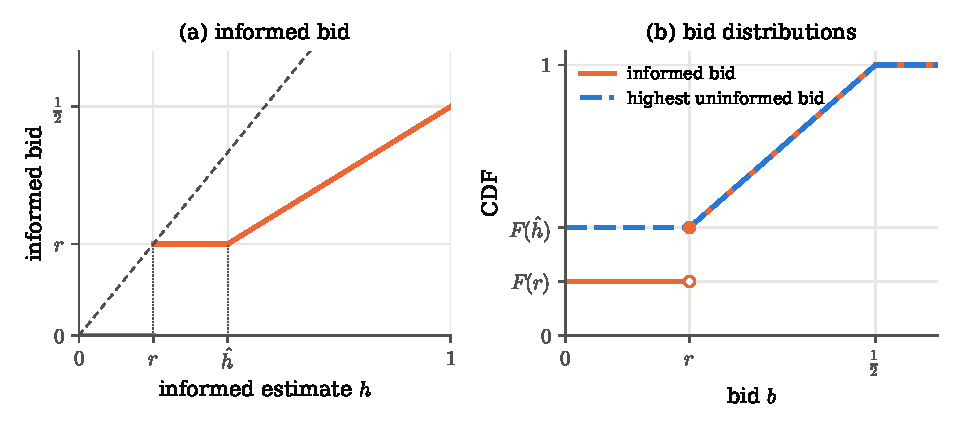
\includegraphics[width=0.95\textwidth]{figures/ch14/emw_equilibrium.pdf}
  \caption{Equilibrium with one informed bidder, for $H$ uniform on $[0,1]$ and reserve price $r=0.2$.
  Panel (a): the informed bid function, which is zero (no bid) below $r$, equal to $r$ on $[r,\hat h]$ with
  $\hat h=0.4$, and $\frac{h}{2}$ above $\hat h$. Panel (b): the distribution functions of the informed bid and
  of the highest uninformed bid. They coincide above $r$ and differ only in their masses at zero and at
  $r$.}\label{fig:14-emw}
\end{figure}

A numerical example makes the predictions concrete (\cref{fig:14-emw}). Let $H$ be uniform on $[0,1]$ and
$r=0.2$. Then $\E[H\mid H<\hat h]=\frac{\hat h}{2}=r$ gives $\hat h=0.4$, and $\sigma^*(h)=\frac{h}{2}$ for
$h>0.4$. The uninformed bidders abstain with probability $0.4$, and otherwise their highest bid has
distribution function $G^*(b)=2b$ on $(0.2,0.5]$. The informed bidder wins half of all auctions and $0.5435$
of the auctions with a bid, by \eqref{eq:14-hp-winprob}. Its expected profit is
$\int_{0.4}^1\frac{h}{2}\,h\,dh+0.4\int_{0.2}^{0.4}(h-0.2)\,dh=0.156+0.008=0.164$. The tract is sold unless
$H<r$ and no uninformed bidder bids, so expected surplus is $0.5-0.2\times0.4\times0.1=0.492$. The seller's
expected revenue is $0.492-0.164=0.328$. The uninformed bidders lose $0.15$ per tract on the tracts where the
informed bidder abstains and gain $0.0375$ per tract on the others, which nets to zero. These numbers come from
the script \texttt{emw\_example.py}, which also confirms them by simulation.

\Cref{prop:14-mw-garbling,prop:14-emw} make the same point from two sides. A bidder whose information is a
garbling of a rival's information earns nothing, and a bidder with exclusive information earns a rent even
against many rivals. The value of information in an auction lies in its privacy.

\subsection{The English auction}\label{sec:14-mw-english}

Milgrom and Weber model the English auction as the Japanese button auction of
\cref{def:14-button}. The price rises continuously from zero, the price and the number of active bidders are
displayed at all times, and exits are public and irrevocable. When one bidder remains, it wins and pays the
price at which the last rival left. With two bidders the English and second-price auctions are strategically
equivalent (\cref{prop:14-english-spa-n2}). With three or more bidders, the prices at which bidders drop out
convey information to those who remain, and the two formats differ.

Suppose $k$ bidders have quit, at prices $p_1\le\dots\le p_k$. A strategy for bidder $i$ specifies, for each
such history, the price $\beta_k(s_i\mid p_1,\dots,p_k)\ge p_k$ at which it will quit if nobody else quits
first. \citet[eqs.~(5)--(6)]{MilgromWeber1982} define the strategy $\beta^E=(\beta^E_0,\dots,
\beta^E_{n-2})$ iteratively. Before any exit,
\begin{equation}\label{eq:14-mw-english0}
  \beta^E_0(s)=\E\left[V_1\mid S_1=s,\,Y_1=s,\dots,Y_{n-1}=s\right].
\end{equation}
After $k=1,\dots,n-2$ exits,
\begin{equation}\label{eq:14-mw-englishk}
  \beta^E_k(s\mid p_1,\dots,p_k)=\E\left[V_1\mid S_1=s,\,Y_1=\dots=Y_{n-k-1}=s,\,
  Y_{n-k}=y_{n-k},\dots,Y_{n-1}=y_{n-1}\right].
\end{equation}
The signals of the bidders who quit are inferred from their exit prices. They solve
$\beta^E_0(y_{n-1})=p_1$, $\beta^E_1(y_{n-2}\mid p_1)=p_2$, and so on up to
$\beta^E_{k-1}(y_{n-k}\mid p_1,\dots,p_{k-1})=p_k$.

These strategies are myopic in a precise sense \citep[p.~1105]{MilgromWeber1982}. Suppose nobody has quit
and the price has reached $\beta^E_0(y)$. If all other bidders quit at that instant, bidder 1 would infer that
$Y_1=\dots=Y_{n-1}=y$. It would then value the object at $\E[V_1\mid S_1=s,Y_1=\dots=Y_{n-1}=y]$, and its
payoff from winning at the current price would be this value minus $\beta^E_0(y)$. By \cref{prop:14-affil-props}(iii)
the difference is positive if $s>y$ and negative if $s<y$. So $\beta^E_0$ keeps it active until the price
at which it would be just indifferent between winning and losing. The later strategies $\beta^E_k$ have the
same interpretation, with the signals of those who quit inferred from their exit prices.

\begin{proposition}[{\citealp[Theorem~10]{MilgromWeber1982}}]\label{prop:14-mw-english}
Under \cref{ass:14-mw}, the profile in which every bidder uses $\beta^E$ is an equilibrium of the English
auction. If bidder 1 wins, it pays
\begin{equation}\label{eq:14-mw-english-price}
  \bar v(Y_1,Y_1,Y_2,\dots,Y_{n-1}),\qquad\text{where }
  \bar v(s,y_1,\dots,y_{n-1})=\E\left[V_1\mid S_1=s,\,Y_1=y_1,\dots,Y_{n-1}=y_{n-1}\right],
\end{equation}
evaluated at the realized order statistics.
\end{proposition}

\begin{proof}
Each $\beta^E_k$ is increasing in its first argument, by \cref{ass:14-mw}(ii) and
\cref{prop:14-affil-props}(iii). Exits therefore occur in increasing order of signals and reveal them. Let
bidders $2,\dots,n$ use $\beta^E$. While bidder 1 is active, the history of exits consists only of rivals'
exits, so its own strategy affects whether it wins and not the price it pays if it wins. If it outlasts
everyone, the last rival to quit has signal $Y_1$. That rival quits at $\beta^E_{n-2}(Y_1\mid p_1,\dots,p_{n-2})$,
the expected value to a bidder with signal $Y_1$ given that the other remaining bidder also has signal $Y_1$
and given the revealed signals $Y_2,\dots,Y_{n-1}$. By the symmetry of $u$ this equals
$\bar v(Y_1,Y_1,Y_2,\dots,Y_{n-1})$, which proves \eqref{eq:14-mw-english-price}.

Given its own signal and the rivals' signals, bidder 1 values the object at
$\bar v(s,Y_1,\dots,Y_{n-1})$ in expectation. Its payoff from winning is therefore
\begin{equation*}
  \bar v(s,Y_1,Y_2,\dots,Y_{n-1})-\bar v(Y_1,Y_1,Y_2,\dots,Y_{n-1}),
\end{equation*}
which is nonnegative if and only if $s\ge Y_1$, by monotonicity of $\bar v$ in its first argument. Under
$\beta^E$ it wins exactly when $s>Y_1$ (the event $s=Y_1$ has probability zero). It thus wins in every
realization in which winning is profitable and in no other. No strategy can do better.
\end{proof}

The argument is pointwise. Bidder 1 would not regret its strategy even if it learned all rivals' signals,
so the equilibrium is an \emph{ex post equilibrium} \citep[Chapter~6]{Krishna2010}. With private values,
$\beta^E_k(s\mid\cdot)=s$ for every $k$, and the strategy reduces to staying in until the price reaches one's
value, as in \citet[eq.~(2.6)]{AtheyHaile2007} and \cref{sec:14-spa}.

With common values the equilibrium is not unique. \citet{BikhchandaniHaileRiley2002} show that there are
many symmetric equilibria in strictly increasing, weakly undominated strategies, even with symmetric bidders.
In every such equilibrium, a bidder who is one of the last two to exit quits at
\begin{equation*}
  \E\left[V_i\mid S_i=s_i,\ S_j=s_i\text{ for active }j\ne i,\ S_k=s_k\text{ for }k\in\mathcal E_i\right],
\end{equation*}
where $\mathcal E_i$ is the set of bidders who quit before it \citep[eq.~(2.7)]{AtheyHaile2007}. The
Milgrom-Weber equilibrium is the one in which every bidder follows this rule at every stage. The multiplicity
concerns the earlier exits, those below the final price, so these exit prices have no unique interpretation. This complicates the use
of losing bids in empirical work (\cref{ch:auction-empirics}).

\begin{example}[Mineral rights, continued]\label{ex:14-mineral-english}
In \cref{ex:14-mineral}, the posterior of $V$ given any set of signals is uniform on
$[\max_is_i-\omega,\ \min_is_i+\omega]$, so the posterior mean is the midpoint of the highest and lowest
signals. Before anyone quits all signals in \eqref{eq:14-mw-english0} equal $s$, so $\beta^E_0(s)=s$. After
$k\ge1$ exits the highest signal in \eqref{eq:14-mw-englishk} is $s$ and the lowest is $y_{n-1}$, so
$\beta^E_k(s\mid\cdot)=\frac{s+y_{n-1}}{2}$. The lowest bidder quits at its signal. The others then stay in
until the midpoint between their own signal and that lowest signal. For $n\ge3$ the winner pays
$\frac{Y_1+Y_{n-1}}{2}$, the midpoint of the second-highest and the lowest signal. For $n=2$ it pays $Y_1$.
\end{example}

\subsection{The first-price auction}\label{sec:14-mw-fpa}

We first derive the necessary conditions for a symmetric equilibrium with an increasing, differentiable bid
function $\beta$ \citep[p.~1106, following \citealp{Wilson1977}]{MilgromWeber1982}. Suppose bidders
$2,\dots,n$ use $\beta$. If bidder 1 has signal $s$ and bids $b$, its expected payoff is
\begin{align*}
  \Pi(b;s)&=\E\left[(V_1-b)\indic\{\beta(Y_1)<b\}\mid S_1=s\right]\\
  &=\E\left[\E\left[(V_1-b)\indic\{\beta(Y_1)<b\}\mid S_1,Y_1\right]\mid S_1=s\right]\\
  &=\E\left[\left(v(S_1,Y_1)-b\right)\indic\{\beta(Y_1)<b\}\mid S_1=s\right]\\
  &=\int_{\underline s}^{\beta^{-1}(b)}\left(v(s,\alpha)-b\right)f_{Y_1}(\alpha\mid s)\,d\alpha.
\end{align*}
Differentiating with respect to $b$ by Leibniz's rule,
\begin{equation*}
  \Pi_b(b;s)=\frac{\left(v(s,\beta^{-1}(b))-b\right)f_{Y_1}(\beta^{-1}(b)\mid s)}{\beta'(\beta^{-1}(b))}
  -F_{Y_1}(\beta^{-1}(b)\mid s).
\end{equation*}
In equilibrium $\Pi_b(\beta(s);s)=0$. Substituting $b=\beta(s)$ and rearranging yields the linear
differential equation \citep[eq.~(7)]{MilgromWeber1982}
\begin{equation}\label{eq:14-mw-ode}
  \beta'(s)=\left(v(s,s)-\beta(s)\right)\frac{f_{Y_1}(s\mid s)}{F_{Y_1}(s\mid s)}.
\end{equation}
Two further necessary conditions fix the boundary. First, $v(s,s)-\beta(s)\ge0$ for every $s$. Otherwise the
payoff $\int_{\underline s}^s(v(s,\alpha)-\beta(s))f_{Y_1}(\alpha\mid s)\,d\alpha$ would be negative, since
$v(s,\alpha)\le v(s,s)$ for $\alpha\le s$, and bidding zero would do better. Second,
$v(\underline s,\underline s)-\beta(\underline s)\le0$. Otherwise the lowest type could raise its bid slightly
above $\beta(\underline s)$, win against rivals with low signals, and earn a positive payoff instead of zero.
Together these give the boundary condition $\beta(\underline s)=v(\underline s,\underline s)$.

\begin{proposition}[{\citealp[Theorem~14]{MilgromWeber1982}}]\label{prop:14-mw-fpa}
Under \cref{ass:14-mw}, the strategy
\begin{equation}\label{eq:14-mw-fpa-bid}
  \beta^{FP}(s)=\int_{\underline s}^{s}v(\alpha,\alpha)\,dL(\alpha\mid s),
  \qquad
  L(\alpha\mid s)=\exp\left(-\int_\alpha^s\frac{f_{Y_1}(t\mid t)}{F_{Y_1}(t\mid t)}\,dt\right),
\end{equation}
used by every bidder is a symmetric equilibrium of the first-price auction. Equivalently,
\begin{equation}\label{eq:14-mw-fpa-bid2}
  \beta^{FP}(s)=v(s,s)-\int_{\underline s}^sL(\alpha\mid s)\,dv(\alpha,\alpha).
\end{equation}
\end{proposition}

We follow Milgrom and Weber's conventions. The ratio $\frac{f_{Y_1}(t\mid t)}{F_{Y_1}(t\mid t)}$ is zero
outside the support of $Y_1$, and $L(\alpha\mid s)=0$ when the integral is infinite (their footnotes 22 and
23). We read $L(\cdot\mid s)$ as a distribution function on $[\underline s,s]$ that places any mass
$L(\underline s\mid s)$ at $\underline s$, and the integral in \eqref{eq:14-mw-fpa-bid} includes that atom.

\begin{proof}
Write $\zeta(t)=\frac{f_{Y_1}(t\mid t)}{F_{Y_1}(t\mid t)}$.

\emph{Solving the equation.} Rewrite \eqref{eq:14-mw-ode} as $\beta'(s)+\zeta(s)\beta(s)=\zeta(s)v(s,s)$. Fix an
interior point $s_0$ and let $\Gamma(s)=\int_{s_0}^s\zeta(t)\,dt$. Multiplying by the integrating factor
$e^{\Gamma(s)}$ gives
\begin{equation*}
  \frac{d}{ds}\left[\beta(s)e^{\Gamma(s)}\right]=\zeta(s)v(s,s)e^{\Gamma(s)}.
\end{equation*}
Integrating from $\underline s$ to $s$,
\begin{equation*}
  \beta(s)e^{\Gamma(s)}=\beta(\underline s)e^{\Gamma(\underline s)}
  +\int_{\underline s}^s\zeta(\alpha)v(\alpha,\alpha)e^{\Gamma(\alpha)}\,d\alpha.
\end{equation*}
Divide by $e^{\Gamma(s)}$. Note that $L(\alpha\mid s)=e^{\Gamma(\alpha)-\Gamma(s)}$ and
$\frac{\partial L(\alpha\mid s)}{\partial\alpha}=\zeta(\alpha)L(\alpha\mid s)$. Imposing
$\beta(\underline s)=v(\underline s,\underline s)$,
\begin{equation*}
  \beta(s)=v(\underline s,\underline s)L(\underline s\mid s)
  +\int_{\underline s}^sv(\alpha,\alpha)\frac{\partial L(\alpha\mid s)}{\partial\alpha}\,d\alpha,
\end{equation*}
which is \eqref{eq:14-mw-fpa-bid} with the atom at $\underline s$. Integrating the second term by parts and
using $L(s\mid s)=1$,
\begin{equation*}
  \int_{\underline s}^sv(\alpha,\alpha)\frac{\partial L(\alpha\mid s)}{\partial\alpha}\,d\alpha
  =v(s,s)-v(\underline s,\underline s)L(\underline s\mid s)-\int_{\underline s}^sL(\alpha\mid s)\,dv(\alpha,\alpha).
\end{equation*}
The atom term cancels, which gives \eqref{eq:14-mw-fpa-bid2}.

\emph{Monotonicity.} As a function of $\alpha$, $L(\cdot\mid s)$ is nondecreasing with $L(s\mid s)=1$, so it is a
distribution function on $[\underline s,s]$. It increases stochastically in $s$. For $s'>s$ and $\alpha\le s$,
$L(\alpha\mid s')=L(\alpha\mid s)\exp(-\int_s^{s'}\zeta)\le L(\alpha\mid s)$, and for $\alpha\in(s,s']$,
$L(\alpha\mid s')\le1=L(\alpha\mid s)$ once we extend $L(\cdot\mid s)$ by one above $s$. Since
$v(\alpha,\alpha)$ is nondecreasing, its mean under $L(\cdot\mid s)$ rises with $s$, so $\beta^{FP}$ is
nondecreasing. Where $v(s,s)>\beta^{FP}(s)$, \eqref{eq:14-mw-ode} shows that it is strictly increasing.

\emph{Sufficiency.} Assume for now that $\beta=\beta^{FP}$ is continuous, and hence differentiable after a monotone
rescaling of signals (\cref{prop:14-affil-props}(i)). A bidder with signal $z$ need only consider bids in
the range of $\beta$, since higher bids are dominated by $\beta(\bar s)$ and lower bids never win. Let its bid be
$\beta(x)$. Substituting $b=\beta(x)$ into $\Pi_b$ and factoring,
\begin{equation*}
  \Pi_b(\beta(x);z)=\frac{f_{Y_1}(x\mid z)}{\beta'(x)}
  \left[\left(v(z,x)-\beta(x)\right)-\beta'(x)\frac{F_{Y_1}(x\mid z)}{f_{Y_1}(x\mid z)}\right].
\end{equation*}
At $z=x$ the bracket is zero by \eqref{eq:14-mw-ode}. Take $x<z$. Then $v(z,x)\ge v(x,x)$ by
\cref{cor:14-mw-v}, and $\frac{F_{Y_1}(x\mid z)}{f_{Y_1}(x\mid z)}\le\frac{F_{Y_1}(x\mid x)}{f_{Y_1}(x\mid x)}$
by \cref{lem:14-mw-lemma1}. With $\beta'\ge0$, the bracket is at least
$(v(x,x)-\beta(x))-\beta'(x)\frac{F_{Y_1}(x\mid x)}{f_{Y_1}(x\mid x)}=0$. For $x>z$ both inequalities reverse
and the bracket is at most zero. So the payoff rises in $x$ below $z$ and falls above $z$, and $x=z$ is
optimal.

\emph{Continuity.} \citet[p.~1108]{MilgromWeber1982} show that $\beta^{FP}$ can jump at $x$ only if
$F_{Y_1}(x\mid x+\epsilon)=0$ for every $\epsilon>0$. By affiliation and symmetry this means that if any signal
exceeds $x$, all signals do. The game then splits into two subgames, one in which it is common knowledge that
all signals exceed $x$ and one in which none does. The argument above applies within each.
\end{proof}

A jump can occur \citep[footnote~21]{MilgromWeber1982}. Let $n=2$ and $V_i=S_i$. With probability
$\frac{1}{2}$ both signals are drawn independently and uniformly from $[0,1]$, and with probability
$\frac{1}{2}$ from $[1,2]$. A bidder's signal reveals the regime, and within each regime the auction is the
uniform private values auction of \cref{sec:14-fpa}. The equilibrium bid is $\frac{s}{2}$ on $[0,1)$ and
$1+\frac{s-1}{2}$ on $(1,2]$, so it jumps from $\frac{1}{2}$ to $1$ at $s=1$. The signals remain affiliated,
because conditional on one signal being high the other is more likely to be high.

The first-price formula nests the private values case. With independent signals, $F_{Y_1}(t\mid s)=F(t)^{n-1}$
does not depend on $s$, so $\zeta(t)=\frac{(n-1)f(t)}{F(t)}$ and
\begin{equation*}
  L(\alpha\mid s)=\exp\left(-(n-1)\left[\ln F(s)-\ln F(\alpha)\right]\right)=\frac{F(\alpha)^{n-1}}{F(s)^{n-1}}.
\end{equation*}
This is the distribution function of $Y_1$ conditional on $Y_1\le s$. Hence $\beta^{FP}(s)=\E[v(Y_1,Y_1)\mid
Y_1<s]$ with independent signals. With private values $v(\alpha,\alpha)=\alpha$, and we recover the
Riley-Samuelson bid in its conditional-expectation form \eqref{eq:14-rs-condexp} without a reserve price. With
$V=\frac{S_1+S_2}{2}$ and independent uniform signals, as in \cref{ex:14-iv-independent}, $v(\alpha,\alpha)=\alpha$ again
and $\beta^{FP}(s)=\frac{s}{2}$. With affiliated signals, $L(\cdot\mid s)$ is no longer a conditional
distribution of $Y_1$, and this is where the formats come apart.

\begin{example}[Mineral rights, continued]\label{ex:14-mineral-fpa}
In \cref{ex:14-mineral}, given $S_1=s$ the posterior of $V$ is uniform on $[s-\omega,s+\omega]$, and given $V$
each rival signal falls below $s$ with probability $\frac{s-V+\omega}{2\omega}$. Substituting
$t=s+\omega-V$,
\begin{align*}
  F_{Y_1}(s\mid s)&=\frac{1}{2\omega}\int_0^{2\omega}\left(\frac{t}{2\omega}\right)^{n-1}dt=\frac{1}{n},\\
  f_{Y_1}(s\mid s)&=\frac{1}{2\omega}\int_0^{2\omega}(n-1)\left(\frac{t}{2\omega}\right)^{n-2}\frac{1}{2\omega}\,dt
  =\frac{1}{2\omega}.
\end{align*}
So $\zeta(t)=\frac{n}{2\omega}$ is constant and $L(\alpha\mid s)=e^{-\frac{n(s-\alpha)}{2\omega}}$. With
$v(\alpha,\alpha)=\alpha-\omega\frac{n-2}{n}$ from \eqref{eq:14-mineral-spa}, $dv(\alpha,\alpha)=d\alpha$, and
\eqref{eq:14-mw-fpa-bid2} gives
\begin{equation}\label{eq:14-mineral-fpa}
  \beta^{FP}(s)=s-\omega\frac{n-2}{n}-\int_{-\infty}^se^{-\frac{n(s-\alpha)}{2\omega}}\,d\alpha
  =s-\omega\frac{n-2}{n}-\frac{2\omega}{n}=s-\omega.
\end{equation}
One checks directly that $\beta^{FP\prime}(s)=1=\left(v(s,s)-\beta^{FP}(s)\right)\frac{n}{2\omega}$. The bid
$s-\omega$ never loses money, since $V\ge s-\omega$ for every possible value. With a proper uniform prior the
lower boundary changes the bid, but its effect dies out exponentially in the distance from the bottom. In the
script \texttt{mineral\_rights.py} with $n=3$, the exact bid for a signal five units of $\omega$ above the
bottom of the prior support differs from $s-\omega$ by about $0.001\omega$.
\end{example}

\begin{example}[Affiliated private values, continued]\label{ex:14-apv-fpa}
From \eqref{eq:14-apv-cond}, $f_{Y_1}(t\mid t)=\frac{2(1+t^2)}{2+t}$ and
$F_{Y_1}(t\mid t)=\frac{t(2+t^2)}{2+t}$, so
\begin{equation*}
  \zeta(t)=\frac{2(1+t^2)}{t(2+t^2)}.
\end{equation*}
We decompose by partial fractions, $\frac{2+2t^2}{t(2+t^2)}=\frac{a}{t}+\frac{bt+c}{2+t^2}$. Multiplying out,
$2+2t^2=a(2+t^2)+(bt+c)t=2a+(a+b)t^2+ct$. Matching coefficients gives $a=1$, $c=0$ and $b=1$, so
$\zeta(t)=\frac{1}{t}+\frac{t}{2+t^2}$. Integrating,
\begin{equation*}
  \int_\alpha^s\zeta(t)\,dt=\ln\frac{s}{\alpha}+\frac{1}{2}\ln\frac{2+s^2}{2+\alpha^2},
  \qquad
  L(\alpha\mid s)=\frac{\alpha\sqrt{2+\alpha^2}}{s\sqrt{2+s^2}}.
\end{equation*}
Here $L(0\mid s)=0$, so there is no atom. With private values $v(\alpha,\alpha)=\alpha$, and
\eqref{eq:14-mw-fpa-bid2} gives
\begin{align}
  \beta^{FP}(s)&=s-\frac{1}{s\sqrt{2+s^2}}\int_0^s\alpha\sqrt{2+\alpha^2}\,d\alpha\notag\\
  &=s-\frac{1}{s\sqrt{2+s^2}}\left[\frac{(2+\alpha^2)^{\frac{3}{2}}}{3}\right]_0^s
  =s-\frac{(2+s^2)^{\frac{3}{2}}-2^{\frac{3}{2}}}{3s\sqrt{2+s^2}}.\label{eq:14-apv-fpa}
\end{align}
A symbolic check in \texttt{apv\_example.py} confirms that \eqref{eq:14-apv-fpa} solves \eqref{eq:14-mw-ode}.
As $s\to0$ the ratio $\frac{\beta^{FP}(s)}{s}$ tends to $\frac{1}{2}$, so $\beta^{FP}(0)=0=v(0,0)$. At the top,
$\beta^{FP}(1)=\frac{2\sqrt6}{9}\approx0.544$.

\Cref{fig:14-apv-bids} plots the bids. The first-price bid lies slightly above the benchmark $\frac{s}{2}$
for independent uniform values. A cleaner comparison holds the marginal distribution fixed. With independent
signals and the same marginal density $\frac{2}{5}(2+s)$, the Riley-Samuelson bid is
$\frac{2s(s+3)}{3(s+4)}$. It exceeds the affiliated bid at low signals ($0.1275$ versus $0.1260$ at $s=0.25$)
and falls below it at high signals ($0.533$ versus $0.544$ at $s=1$). A bidder with a high signal expects
strong rivals and bids more aggressively. A bidder with a low signal expects weak rivals and shades more.
\end{example}

\begin{figure}[htbp]
  \centering
  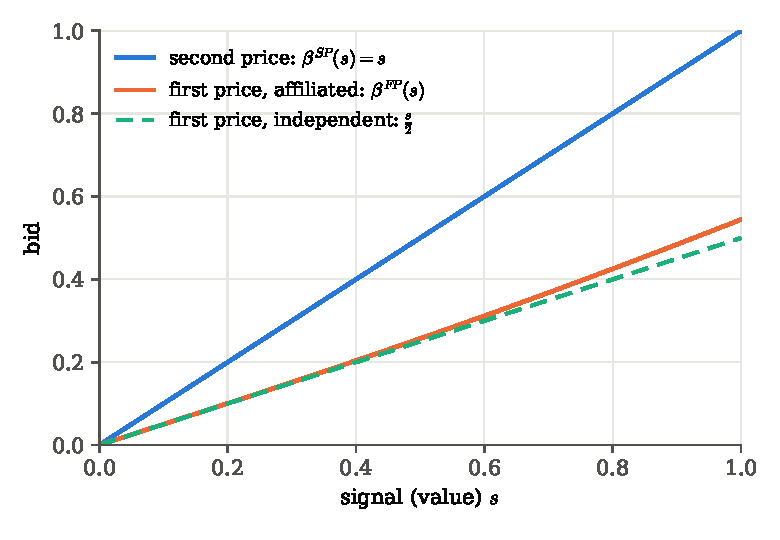
\includegraphics[width=0.72\textwidth]{figures/ch14/apv_bids.pdf}
  \caption{Equilibrium bids for the affiliated private values density $f(s_1,s_2)=\frac{4}{5}(1+s_1s_2)$ on
  $[0,1]^2$ with two bidders. The second-price bid is $s$. The first-price bid is \eqref{eq:14-apv-fpa}. The
  dashed line is the first-price bid $\frac{s}{2}$ for independent uniform values.}\label{fig:14-apv-bids}
\end{figure}

The first-order condition can also be written in terms of the bid distribution, which is the form used for
estimation. Consider affiliated private values, possibly asymmetric, and let $M_i=\max_{j\ne i}B_j$ be the
highest rival bid. Bidder $i$ with value $v_i$ solves
\begin{equation*}
  \max_b\ \E\left[(v_i-b)\indic\{M_i\le b\}\mid V_i=v_i\right]=\max_b\ (v_i-b)\Pr\left(M_i\le b\mid V_i=v_i\right).
\end{equation*}
The conditioning on $v_i$ matters, because under affiliation a bidder's own value is informative about rivals'
values and hence about their bids. The first-order condition is
\begin{equation*}
  -\Pr\left(M_i\le b\mid V_i=v_i\right)+(v_i-b)\frac{\partial\Pr\left(M_i\le b\mid V_i=v_i\right)}{\partial b}=0,
\end{equation*}
which rearranges to
\begin{equation*}
  v_i=b+\frac{\Pr\left(M_i\le b\mid V_i=v_i\right)}{\frac{\partial}{\partial b}\Pr\left(M_i\le b\mid V_i=v_i\right)}.
\end{equation*}
The derivative is taken in the threshold $b$, holding the conditioning value fixed. In an equilibrium with
strictly increasing strategies $\beta_i$, the events $\{V_i=v_i\}$ and $\{B_i=\beta_i(v_i)\}$ coincide. So
$\Pr(M_i\le m\mid V_i=v_i)=G_{M\mid B}(m\mid b_i)$, where $G_{M\mid B}(m\mid b)=\Pr(M_i\le m\mid B_i=b)$ and
$b_i=\beta_i(v_i)$. Let $g_{M\mid B}(m\mid b)$ be its density in $m$. At the equilibrium bid,
\begin{equation}\label{eq:14-apv-foc}
  v_i=b_i+\frac{G_{M\mid B}(b_i\mid b_i)}{g_{M\mid B}(b_i\mid b_i)}.
\end{equation}
Everything on the right side is a feature of the joint distribution of a bidder's own bid and the highest
rival bid, which is observed when all bids are recorded. \Cref{ch:auction-empirics} uses \eqref{eq:14-apv-foc}
to recover values from bids \citep{LiPerrigneVuong2002,CampoPerrigneVuong2003}. With common values the same
argument gives \citet[eq.~(2.4)]{AtheyHaile2007}, in which the left side is the pivotal expected value
$\E[V_i\mid S_i=s_i,\ M_i=\beta(s_i)]$. In the symmetric Milgrom-Weber model this is $v(s,s)$. There,
$G_{M\mid B}(b\mid b)=F_{Y_1}(s\mid s)$ and $g_{M\mid B}(b\mid b)=\frac{f_{Y_1}(s\mid s)}{\beta'(s)}$ at
$b=\beta(s)$, and \eqref{eq:14-apv-foc} becomes \eqref{eq:14-mw-ode}.

Existence and uniqueness of equilibrium are now well understood. The following theorem collects the results
summarized by \citet[Theorem~2.1]{AtheyHaile2007}.

\begin{theorem}[Existence and uniqueness in first-price auctions]\label{thm:14-existence}
Suppose values have a compact, convex common support, signals are affiliated with a product support, and
their joint density is strictly positive on the interior of the support.
\begin{enumerate}[label=(\roman*)]
  \item An equilibrium in pure, nondecreasing strategies exists \citep{Athey2001,RenyZamir2004}. Strategies
  can be taken strictly increasing, except in common values models with asymmetric bidders and dependent
  signals. There, at most one bidder may bid the lowest winning bid with positive probability
  \citep{McAdams2003}.
  \item With private values and either independence or symmetry, and a continuously differentiable density,
  the equilibrium is unique and in pure, strictly increasing, differentiable strategies
  \citep{Lebrun1999,MaskinRiley2003,McAdams2003,McAdams2007}.
  \item With symmetric bidders and a continuously differentiable density, there is a unique equilibrium
  within the class of nondecreasing pure strategies. It is symmetric, strictly increasing and differentiable,
  and it is the equilibrium of \cref{prop:14-mw-fpa} \citep{McAdams2007}.
\end{enumerate}
\end{theorem}

We do not prove the theorem. Existence for asymmetric bidders rests on single-crossing arguments that go
beyond this book. Part (iii) shows that, among monotone equilibria, the Milgrom-Weber first-price
equilibrium is the only one in the symmetric model.

\section{Affiliated Values II: The Linkage Principle, Revenue Ranking, and Information Disclosure}\label{sec:14-mw-rank}

With independent private values the four standard formats raise the same expected revenue
(\cref{prop:14-ret}). Affiliation breaks this equivalence in a systematic direction. This section explains why
through the linkage principle, proves the ranking, and applies the same logic to the seller's disclosure of
information, reserve prices and entry fees. It then asks which results survive risk aversion and closes with
an assessment of the paper.

\subsection{The linkage principle}\label{sec:14-linkage}

\citet[pp.~1110--1111]{MilgromWeber1982} view each auction as a revelation game in which every bidder chooses a
report $x$ in place of a bid $\beta(x)$. No auction can set prices directly in terms of bidders' preferences
and information. Prices can depend only on the reports and on the seller's information. If the price depends
on variables other than the winner's own report, and those variables are affiliated with the winner's signal,
then the price is statistically linked to that signal. The expected price, as a function of the winner's
signal, rises more steeply than it otherwise would. In all three auctions the winner with the lowest signal
expects to pay $v(\underline s,\underline s)$. A steeper expected payment function therefore means higher
prices and lower bidder profits.

To make this precise, consider a symmetric auction mechanism $\mathcal M$ with a symmetric, increasing
equilibrium in which the highest signal wins. For bidder 1 with signal $z$ who bids as if its signal were $x$,
define the expected value it receives,
\begin{equation*}
  R(x,z)=\E\left[V_1\indic\{Y_1<x\}\mid S_1=z\right],
\end{equation*}
and its expected payment conditional on winning, $W^{\mathcal M}(x,z)$. Its expected payoff is
$R(x,z)-W^{\mathcal M}(x,z)F_{Y_1}(x\mid z)$. In equilibrium $x=z$ is optimal, so the first-order condition
holds at $x=z$ \citep[eq.~(9)]{MilgromWeber1982}:
\begin{equation}\label{eq:14-mw-foc9}
  0=R_1(z,z)-W^{\mathcal M}_1(z,z)F_{Y_1}(z\mid z)-W^{\mathcal M}(z,z)f_{Y_1}(z\mid z),
\end{equation}
where subscripts denote partial derivatives. The boundary condition is
$W^{\mathcal M}(\underline s,\underline s)=v(\underline s,\underline s)$. In the first-price auction the
winner pays its own bid, so $W^{FP}(x,z)=\beta^{FP}(x)$. In the second-price auction it pays the highest rival
bid, so $W^{SP}(x,z)=\E[v(Y_1,Y_1)\mid Y_1<x,\,S_1=z]$. The partial derivative $W_2^{\mathcal M}$ measures how
much the expected price depends on the winner's true signal when its report is held fixed. We call it the
\emph{linkage} of the mechanism.

\begin{proposition}[Linkage principle]\label{prop:14-linkage}
Let $\mathcal M$ and $\mathcal M'$ be two mechanisms as above that satisfy \eqref{eq:14-mw-foc9}. Suppose
$W^{\mathcal M}(\underline s,\underline s)=W^{\mathcal M'}(\underline s,\underline s)$ and
$W^{\mathcal M}_2(z,z)\ge W^{\mathcal M'}_2(z,z)$ for all $z$. Then $W^{\mathcal M}(z,z)\ge W^{\mathcal
M'}(z,z)$ for all $z$, and $\mathcal M$ yields an expected revenue at least as large as $\mathcal M'$.
\end{proposition}

\begin{proof}
Let $g(z)=W^{\mathcal M}(z,z)$ and $h(z)=W^{\mathcal M'}(z,z)$. Solving \eqref{eq:14-mw-foc9} for $W_1$ in
each mechanism and subtracting,
\begin{equation*}
  W^{\mathcal M}_1(z,z)-W^{\mathcal M'}_1(z,z)=-\left[g(z)-h(z)\right]\frac{f_{Y_1}(z\mid z)}{F_{Y_1}(z\mid z)}.
\end{equation*}
By the chain rule $g'(z)=W^{\mathcal M}_1(z,z)+W^{\mathcal M}_2(z,z)$, and similarly for $h$. Therefore
\begin{equation*}
  g'(z)-h'(z)=-\left[g(z)-h(z)\right]\frac{f_{Y_1}(z\mid z)}{F_{Y_1}(z\mid z)}
  +\left[W^{\mathcal M}_2(z,z)-W^{\mathcal M'}_2(z,z)\right].
\end{equation*}
If $g(z)<h(z)$, the first term is positive and the second is nonnegative, so $g'(z)\ge h'(z)$. Since
$g(\underline s)=h(\underline s)$, \cref{lem:14-crossing} gives $g\ge h$ everywhere. By symmetry each bidder
wins with probability $\frac{1}{n}$, so expected revenue is
$n\,\E[W(S_1,S_1)\indic\{S_1>Y_1\}]=\E[W(S_1,S_1)\mid S_1>Y_1]$, which is larger under $\mathcal M$.
\end{proof}

The principle explains where bidders' profits come from. A bidder earns a rent because the price cannot
depend on its private signal except through its own report. Every channel that makes the price track its
signal through other affiliated variables reduces that rent. General versions of the principle are in
\citet{Milgrom2004} and \citet[Chapter~7]{Krishna2010}.

\subsection{Revenue ranking}\label{sec:14-mw-ranking}

The ranking rests on one inequality, which also delivers the disclosure results of
\cref{sec:14-mw-disclosure}.

\begin{lemma}[Information raises the second-price expected price]\label{lem:14-mw-info}
Let $\bm Z$ be a random vector such that $(\bm Z,S_1,Y_1)$ are affiliated, and let
$w_{\bm Z}(s,y,\bm z)=\E[V_1\mid S_1=s,\,Y_1=y,\,\bm Z=\bm z]$ be nondecreasing. Then
\begin{equation*}
  \E\left[v(Y_1,Y_1)\mid S_1>Y_1\right]\le\E\left[w_{\bm Z}(Y_1,Y_1,\bm Z)\mid S_1>Y_1\right].
\end{equation*}
\end{lemma}

\begin{proof}
By the law of iterated expectations, for all $x$ and $y$,
\begin{equation*}
  v(x,y)=\E\left[\E[V_1\mid S_1,Y_1,\bm Z]\mid S_1=x,Y_1=y\right]=\E\left[w_{\bm Z}(x,y,\bm Z)\mid S_1=x,Y_1=y\right].
\end{equation*}
Now take $x>y$. Applying this identity at the point $(y,y)$ and then \cref{prop:14-affil-props}(iii) to the
nondecreasing function $w_{\bm Z}(y,y,\cdot)$,
\begin{equation*}
  v(y,y)=\E\left[w_{\bm Z}(y,y,\bm Z)\mid S_1=y,Y_1=y\right]\le\E\left[w_{\bm Z}(y,y,\bm Z)\mid S_1=x,Y_1=y\right].
\end{equation*}
Setting $y=Y_1$ and $x=S_1$ on the event $\{S_1>Y_1\}$ and taking expectations,
\begin{equation*}
  \E\left[v(Y_1,Y_1)\mid S_1>Y_1\right]\le\E\left[\E\left[w_{\bm Z}(Y_1,Y_1,\bm Z)\mid S_1,Y_1\right]\mid S_1>Y_1\right]
  =\E\left[w_{\bm Z}(Y_1,Y_1,\bm Z)\mid S_1>Y_1\right].\qedhere
\end{equation*}
\end{proof}

\begin{proposition}[{\citealp[Theorems~11 and 15]{MilgromWeber1982}}]\label{prop:14-mw-ranking}
Let \cref{ass:14-mw} hold, and consider the equilibria of
\cref{prop:14-mw-english,prop:14-mw-spa,prop:14-mw-fpa}. The expected price in the English auction is at least
that in the second-price auction. The expected price in the second-price auction is at least that in the
first-price and Dutch auctions.
\end{proposition}

\begin{proof}
\emph{Second price versus first price.} Both equilibria satisfy \eqref{eq:14-mw-foc9}, because $x=z$ is optimal in
each. In the first-price auction $W^{FP}(x,z)=\beta^{FP}(x)$ does not depend on $z$, so $W^{FP}_2=0$. In the
second-price auction $W^{SP}(x,z)=\E[v(Y_1,Y_1)\mid Y_1<x,S_1=z]$. Since $(S_1,Y_1)$ are affiliated, $v$ is
nondecreasing and the event $\{Y_1<x\}$ is an interval, \cref{prop:14-affil-props}(iii) shows that $W^{SP}$
is nondecreasing in $z$, so $W^{SP}_2\ge0$. Both mechanisms satisfy the boundary condition
$W(\underline s,\underline s)=v(\underline s,\underline s)$. \Cref{prop:14-linkage} gives
$W^{SP}(z,z)\ge W^{FP}(z,z)$ for all $z$, and the expected prices are $\E[W(S_1,S_1)\mid S_1>Y_1]$.

\emph{English versus second price.} When bidder 1 wins, it pays $\bar v(Y_1,Y_1,Y_2,\dots,Y_{n-1})$ in the English
auction (\cref{prop:14-mw-english}) and $v(Y_1,Y_1)$ in the second-price auction. Apply \cref{lem:14-mw-info}
with $\bm Z=(Y_2,\dots,Y_{n-1})$. Then $w_{\bm Z}=\bar v$, which is nondecreasing by \cref{cor:14-mw-v}, and
$(S_1,Y_1,\dots,Y_{n-1})$ are affiliated by \cref{prop:14-affil-props}(iv) and (ii).

\emph{Dutch versus first price.} The two are strategically equivalent (\cref{prop:14-dutch-fpa}).
\end{proof}

The English auction proceeds in two phases \citep[p.~1105]{MilgromWeber1982}. In the first, the $n-2$
bidders with the lowest signals reveal them publicly by dropping out. In the second, the last two bidders play
what amounts to a second-price auction with this public information. \Cref{lem:14-mw-info} says that public
information affiliated with the bidders' signals raises the expected second-price price. The first phase
therefore raises the expected price above the second-price level. In the language of linkage, the English
price is linked to the signals of all losing bidders. The second-price price is linked only to the highest
losing signal, and the first-price price to no other signal at all.

\begin{figure}[htbp]
  \centering
  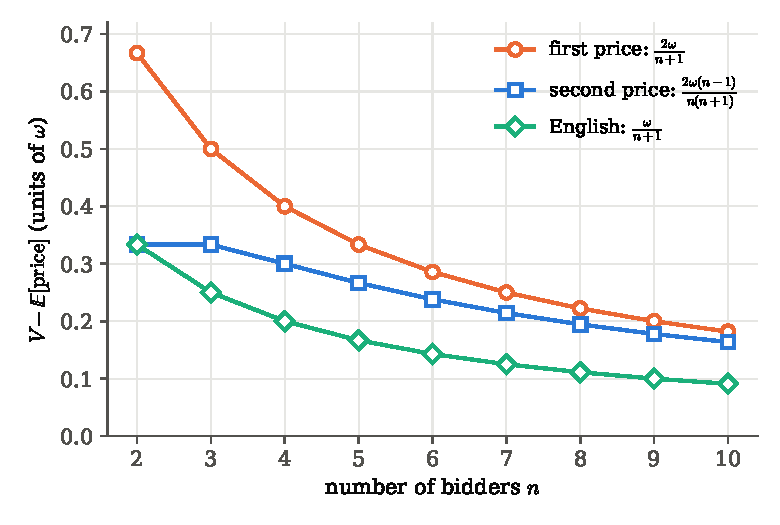
\includegraphics[width=0.72\textwidth]{figures/ch14/mw_mineral_rents.pdf}
  \caption{Expected bidder rents $V-\E[\text{price}]$, in units of $\omega$, in the mineral rights model with
  uniform noise (\cref{ex:14-mineral}) and a diffuse prior. The formulas are derived in the text, and a
  Monte Carlo check is in \texttt{mineral\_rights.py}.}\label{fig:14-mw-ranking}
\end{figure}

The mineral rights example (\cref{ex:14-mineral,ex:14-mineral-english,ex:14-mineral-fpa}) makes the ranking
explicit. Write $S_i=V+\omega(2U_i-1)$ with $U_i$ \iid\ uniform on $[0,1]$. The $k$-th lowest of $n$ uniforms
has mean $\frac{k}{n+1}$, so the $k$-th lowest signal has mean
\begin{equation*}
  \E\left[S_{(k:n)}\right]=V+\omega\left(\frac{2k}{n+1}-1\right)=V+\omega\,\frac{2k-n-1}{n+1}.
\end{equation*}
The first-price winner pays $S_{(n:n)}-\omega$, by \eqref{eq:14-mineral-fpa}. Its expected payment is
\begin{equation*}
  V+\omega\,\frac{n-1}{n+1}-\omega=V-\frac{2\omega}{n+1}.
\end{equation*}
The second-price winner pays $v(S_{(n-1:n)},S_{(n-1:n)})=S_{(n-1:n)}-\omega\frac{n-2}{n}$, by
\eqref{eq:14-mineral-spa}. Its expected payment is
\begin{equation*}
  V+\omega\,\frac{n-3}{n+1}-\omega\,\frac{n-2}{n}
  =V+\omega\,\frac{n(n-3)-(n-2)(n+1)}{n(n+1)}
  =V-\frac{2\omega(n-1)}{n(n+1)}.
\end{equation*}
The English winner pays $\frac{S_{(n-1:n)}+S_{(1:n)}}{2}$, with expectation
\begin{equation*}
  V+\frac{\omega}{2}\left(\frac{n-3}{n+1}+\frac{1-n}{n+1}\right)=V-\frac{\omega}{n+1}.
\end{equation*}
The expected bidder rents are therefore $\frac{2\omega}{n+1}$, $\frac{2\omega(n-1)}{n(n+1)}$ and
$\frac{\omega}{n+1}$. They are ranked as \cref{prop:14-mw-ranking} predicts, because $1\ge\frac{n-1}{n}$ and
$2(n-1)\ge n$. The English and second-price auctions tie at $n=2$, as they must. \Cref{fig:14-mw-ranking}
plots the rents. The first-price rent is twice the English rent for every $n$.

The affiliated private values example (\cref{ex:14-apv,ex:14-apv-fpa}) shows that interdependent values are
not needed. The second-price (and English) revenue is $\E[\min\{S_1,S_2\}]$. By symmetry,
\begin{equation*}
  \E[\min\{S_1,S_2\}]=2\int_0^1\int_0^{s_1}s_2\,\frac{4}{5}(1+s_1s_2)\,ds_2\,ds_1
  =\frac{8}{5}\int_0^1\left(\frac{s_1^2}{2}+\frac{s_1^4}{3}\right)ds_1=\frac{8}{5}\cdot\frac{7}{30}=\frac{28}{75}
  \approx0.3733.
\end{equation*}
We compute the first-price revenue $\E[\beta^{FP}(\max\{S_1,S_2\})]$ by numerical integration and obtain
$0.3676$. The gap is small because the correlation is only $0.054$, but its sign is the one the theory
predicts. Compare \cref{ex:14-iv-independent}, which has interdependent values $V=\frac{S_1+S_2}{2}$
and independent uniform signals. There both formats raise $\frac{1}{3}$. The ranking comes from the
affiliation of the signals. Interdependence of values alone does not produce it. \Cref{tab:14-mw-examples}
collects the numbers.

\begin{table}[htbp]
  \centering
  \caption{Equilibrium bids and expected revenue in the two running examples}\label{tab:14-mw-examples}
  \small
  \renewcommand{\arraystretch}{1.35}
  \begin{tabularx}{\textwidth}{@{}lXcc@{}}
    \toprule
    \multicolumn{4}{@{}l}{\textit{Panel A. Mineral rights with uniform noise, diffuse prior}}\\
    \midrule
    Format & Bid or price & $V-\E[\text{price}]$ & $n=3$\\
    \midrule
    First price & bid $s-\omega$ & $\frac{2\omega}{n+1}$ & $0.500\omega$\\[2pt]
    Second price & bid $s-\omega\frac{n-2}{n}$ & $\frac{2\omega(n-1)}{n(n+1)}$ & $0.333\omega$\\[2pt]
    English & price $\frac{Y_1+Y_{n-1}}{2}$ & $\frac{\omega}{n+1}$ & $0.250\omega$\\[2pt]
    Second price, $S_0$ disclosed & bid $w(s,s,s_0)$ & numerical & $0.192\omega$\\[2pt]
    English, $S_0$ disclosed & price $\frac{\max\{Y_1,S_0\}+\min\{Y_{n-1},S_0\}}{2}$ &
      $\frac{n\omega}{(n+1)(n+2)}$ & $0.150\omega$\\
    \midrule
    \multicolumn{4}{@{}l}{\textit{Panel B. Affiliated private values, $f(s_1,s_2)=\frac{4}{5}(1+s_1s_2)$, $n=2$}}\\
    \midrule
    Format & Bid & Revenue & Bidder surplus\\
    \midrule
    First price & \eqref{eq:14-apv-fpa} & $0.3676$ & $0.3257$\\
    Second price, English & $s$ & $\frac{28}{75}\approx0.3733$ & $0.3200$\\
    Independent uniform values & $\frac{s}{2}$ (first), $s$ (second) & $\frac{1}{3}$ & $\frac{1}{3}$\\
    \bottomrule
  \end{tabularx}

  \smallskip
  \begin{minipage}{\textwidth}
  \footnotesize Notes: In Panel A the seller's signal is $S_0=V+\epsilon_0$ with $\epsilon_0$ uniform on
  $[-\omega,\omega]$ and independent of the bidders' noise. The closed forms are derived in the text. The
  disclosed second-price rent is computed by numerical integration ($0.167\omega$, $0.192\omega$,
  $0.191\omega$ and $0.182\omega$ for $n=2,\dots,5$). In Panel B, expected total surplus is
  $\E[\max\{S_1,S_2\}]=\frac{52}{75}$ with affiliation and $\frac{2}{3}$ with independent uniform values.
  The first-price revenue is computed by numerical integration. Source: scripts \texttt{mineral\_rights.py}
  and \texttt{apv\_example.py}.
  \end{minipage}
\end{table}

\Cref{tab:14-mw-theorems} maps the paper's results to the places where this chapter states and proves them.

\begin{table}[htbp]
  \centering
  \caption{The results of Milgrom and Weber (1982) and where this chapter treats them}\label{tab:14-mw-theorems}
  \small
  \begin{tabularx}{\textwidth}{@{}lXl@{}}
    \toprule
    Result & Content & In this chapter\\
    \midrule
    Theorem 0 & Revenue equivalence with independent private values & \cref{prop:14-ret}\\
    Theorem 1 & Characterization of affiliation, products & \cref{prop:14-affil-char}\\
    Theorems 2--5 & Order statistics, monotone maps, marginals, conditional means & \cref{prop:14-affil-props}\\
    Lemma 1 & $\frac{F_{Y_1}(y\mid z)}{f_{Y_1}(y\mid z)}$ is nonincreasing in $z$ & \cref{lem:14-mw-lemma1}\\
    Theorem 6 & Second-price equilibrium $v(s,s)$ & \cref{prop:14-mw-spa}\\
    Theorem 7 & Garbled information earns nothing & \cref{prop:14-mw-garbling}\\
    Theorems 8, 12, 16 & Disclosure of $S_0$ raises second-price, English, first-price revenue &
      \cref{prop:14-mw-disclosure}\\
    Theorems 9, 13, 17 & No reporting policy beats full disclosure & \cref{prop:14-mw-fullreport}\\
    Theorem 10 & English equilibrium & \cref{prop:14-mw-english}\\
    Theorem 11 & English at least second price & \cref{prop:14-mw-ranking}\\
    Theorem 14 & First-price equilibrium & \cref{prop:14-mw-fpa}\\
    Lemma 2 & Crossing lemma & \cref{lem:14-crossing}\\
    Theorem 15 & Second price at least first price & \cref{prop:14-mw-ranking}\\
    Theorem 18 & Disclosure with an adjusted reserve price & \cref{prop:14-mw-reserve-info}\\
    Theorem 19 & Higher entry fee, lower reserve at a fixed screening level & \cref{prop:14-mw-fee}\\
    Theorem 20 & Information raises willingness to pay only under constant absolute risk aversion &
      \cref{prop:14-mw-cara}\\
    Theorem 21 & Disclosure and ranking under constant absolute risk aversion & \cref{prop:14-mw-cara-disclosure}\\
    Theorems 22--24 & Association and the general definition of affiliation & \cref{sec:14-mw-affil}\\
    \bottomrule
  \end{tabularx}
\end{table}

\subsection{Information disclosure by the seller}\label{sec:14-mw-disclosure}

Suppose the seller observes a variable $S_0$ that is affiliated with $(\bm A,\bm S)$, such as an expert
appraisal. Can the seller gain by revealing it? We assume that the seller can commit to a reporting policy and that its
reports are credible. Credibility is plausible if a buyer has recourse after a false announcement,
or if the seller is an institution, such as an auction house, that values its reputation for truthfulness
\citep[footnote~18]{MilgromWeber1982}.

Define $w(s,y,s_0)=\E[V_1\mid S_1=s,\,Y_1=y,\,S_0=s_0]$, which is nondecreasing by
\cref{prop:14-affil-props}(iii). After $S_0=s_0$ is announced, the conditional density of $(\bm A,\bm S)$ given
$s_0$ is proportional to $f(\bm a,\bm s,s_0)$ with $s_0$ held fixed. It satisfies \eqref{eq:14-affil-ineq}, since
the inequality for $f$ holds in particular for pairs of points with the same value of $s_0$. So the analysis of
\cref{sec:14-mw-eq} applies conditionally. In the second-price auction the equilibrium bid becomes
$\beta^{SP}(s;s_0)=w(s,s,s_0)$, a function of both private and public information
\citep[p.~1102]{MilgromWeber1982}.

\begin{proposition}[{\citealp[Theorems~8, 12 and 16]{MilgromWeber1982}}]\label{prop:14-mw-disclosure}
Let \cref{ass:14-mw} hold, and let $S_0$ be affiliated with $(\bm A,\bm S)$.
\begin{enumerate}[label=(\roman*)]
  \item In the second-price auction, the expected price without disclosure,
  $\mathcal R^{SP}_N=\E[v(Y_1,Y_1)\mid S_1>Y_1]$, is at most the expected price with public disclosure of
  $S_0$, $\mathcal R^{SP}_I=\E[w(Y_1,Y_1,S_0)\mid S_1>Y_1]$.
  \item In the English auction, the expected price without disclosure,
  $\mathcal R^E_N=\E[\bar v(Y_1,Y_1,Y_2,\dots,Y_{n-1})\mid S_1>Y_1]$, is at most the expected price with
  disclosure, $\mathcal R^E_I=\E[\bar w(Y_1,Y_1,Y_2,\dots,Y_{n-1},S_0)\mid S_1>Y_1]$, where
  $\bar w(s,y_1,\dots,y_{n-1},s_0)=\E[V_1\mid S_1=s,\,Y_1=y_1,\dots,Y_{n-1}=y_{n-1},\,S_0=s_0]$.
  \item In the first-price auction, public disclosure of $S_0$ cannot lower, and may raise, the expected price.
\end{enumerate}
\end{proposition}

\begin{proof}
\emph{Part (i).} By symmetry the expected price equals the expected price paid by bidder 1 when it wins, which is
$v(Y_1,Y_1)$ without disclosure and $w(Y_1,Y_1,S_0)$ with it. Apply \cref{lem:14-mw-info} with $\bm Z=S_0$.
The vector $(S_0,S_1,Y_1)$ is affiliated by \cref{prop:14-affil-props}(iv) and (ii), with $S_0$ counted
among the variables $\bm A$, and $w$ is nondecreasing.

\emph{Part (ii).} The argument of \cref{lem:14-mw-info} goes through with $(Y_2,\dots,Y_{n-1})$ added to every
conditioning set. For $x>y_1$,
\begin{align*}
  \bar v(y_1,y_1,y_2,\dots,y_{n-1})
  &=\E\left[\bar w(y_1,y_1,\dots,y_{n-1},S_0)\mid S_1=y_1,Y_1=y_1,\dots\right]\\
  &\le\E\left[\bar w(y_1,y_1,\dots,y_{n-1},S_0)\mid S_1=x,Y_1=y_1,\dots\right],
\end{align*}
where the dots stand for $Y_2=y_2,\dots,Y_{n-1}=y_{n-1}$. Taking expectations over $\{S_1>Y_1\}$ gives the
result.

\emph{Part (iii), sketch.} Let $\beta(\cdot;s_0)$ be the first-price equilibrium after $S_0=s_0$ is announced. It
solves the analogue of \eqref{eq:14-mw-ode} with $w(s,s,s_0)$ in place of $v(s,s)$ and the ratio
$\zeta(s;s_0)=\frac{f_{Y_1}(s\mid s,s_0)}{F_{Y_1}(s\mid s,s_0)}$, with boundary value
$w(\underline s,\underline s,s_0)$. A variant of \cref{lem:14-mw-lemma1} shows that $\zeta(s;s_0)$ is
nondecreasing in $s_0$, and $w$ is nondecreasing in $s_0$. For $s_0'>s_0$, let $g=\beta(\cdot;s_0')$ and
$h=\beta(\cdot;s_0)$. Then $g(\underline s)\ge h(\underline s)$, and $g(x)<h(x)$ implies
$g'(x)=(w(x,x,s_0')-g(x))\zeta(x;s_0')\ge(w(x,x,s_0)-h(x))\zeta(x;s_0)=h'(x)$. By
\cref{lem:14-crossing}, $\beta(x;s_0)$ is nondecreasing in $s_0$. Now define
$W^*(x,z)=\E[\beta(x;S_0)\mid Y_1<x,\,S_1=z]$, the expected payment of a winner with signal $z$ who bids as
if $x$ whatever $S_0$ turns out to be. By \cref{prop:14-affil-props}(iii), $W^*_2\ge0=W^{FP}_2$. The boundary
value is $W^*(\underline s,\underline s)=\E[w(\underline s,\underline s,S_0)\mid Y_1=S_1=\underline s]
=v(\underline s,\underline s)$. A bidder who commits to the report $x$ before $S_0$ is announced chooses
$x=z$, because $x=z$ is optimal for every realization of $S_0$. So $W^*$ satisfies \eqref{eq:14-mw-foc9}.
\Cref{prop:14-linkage} gives $W^*(z,z)\ge\beta^{FP}(z)$, and the expected price is higher with
disclosure.
\end{proof}

Could the seller do better by censoring, that is, reporting $S_0$ only when it is favorable? No. If the policy
is known, rational bidders interpret the absence of a report as bad news. More generally, let the seller's
report be $S_0'=\varrho(S_0,Z)$, where $Z$ is uniform on $[0,1]$ and independent of everything else. The
report may depend both on the seller's information and on the spin of a roulette wheel. Since the policy is
known, we can assume without loss that the seller always makes some report, possibly a blank page
\citep[p.~1103]{MilgromWeber1982}.

\begin{proposition}[{\citealp[Theorems~9, 13 and 17]{MilgromWeber1982}}]\label{prop:14-mw-fullreport}
In the second-price, English and first-price auctions, no reporting policy yields a higher expected price
than always reporting $S_0$.
\end{proposition}

\begin{proof}
Let $g(s_0'\mid s_0)$ be the conditional density of the report given $S_0$ and $g(s_0')$ its marginal. Given
$S_0'=s_0'$, the conditional density of $(\bm A,\bm S,S_0)$ is
$\frac{f(\bm a,\bm s,s_0)\,g(s_0'\mid s_0)}{g(s_0')}$ \citep[footnote~19]{MilgromWeber1982}. For fixed
$s_0'$, this is the product of the affiliated density $f$ and a nonnegative function of $s_0$ alone. A function
of one variable satisfies \eqref{eq:14-affil-ineq} with equality, so the product is affiliated by
\cref{prop:14-affil-char}. Conditional on $S_0'=s_0'$, \cref{prop:14-mw-disclosure} therefore says that
revealing $S_0$ as well raises the expected price. Revealing both $S_0$ and $S_0'$ leads to the same bidding as
revealing $S_0$ alone, because $S_0'$ carries no information about $(\bm A,\bm S)$ beyond $S_0$. Averaging over
$S_0'$ completes the proof.
\end{proof}

Full disclosure links the price to $S_0$, a variable affiliated with the winner's signal that the winner
cannot influence. It dilutes the winner's informational advantage and so lowers its rent
\citep[p.~1117]{MilgromWeber1982}. The results offer an explanation for the expert appraisals and catalog
estimates that reputable auction houses publish.

The mineral rights example quantifies the effect (Panel A of \cref{tab:14-mw-examples}). Let the seller observe
$S_0=V+\epsilon_0$, with $\epsilon_0$ uniform on $[-\omega,\omega]$ and independent of the bidders' noise. In
the English auction with $S_0$ public, the posterior of $V$ at the last exit is uniform. Its support runs from
the largest signal minus $\omega$ to the smallest signal plus $\omega$, where $S_0$ now counts as a signal.
The winner pays
$\frac{\max\{Y_1,S_0\}+\min\{Y_{n-1},S_0\}}{2}$. In uniform units, $\min\{U_{(1:n)},U_0\}$ is the minimum of
$n+1$ uniforms, with mean $\frac{1}{n+2}$. The maximum $\max\{U_{(n-1:n)},U_0\}$ has distribution function
$x\Lambda_n(x)$, where $\Lambda_n(x)=nx^{n-1}(1-x)+x^n$ is the distribution function of $U_{(n-1:n)}$. Its
mean is
\begin{equation*}
  1-\int_0^1x\Lambda_n(x)\,dx=1-n\left(\frac{1}{n+1}-\frac{1}{n+2}\right)-\frac{1}{n+2}
  =1-\frac{2n+1}{(n+1)(n+2)}.
\end{equation*}
Converting back with $S=V+\omega(2U-1)$, the price is
\begin{equation*}
  V+\omega\left(\max\{U_{(n-1:n)},U_0\}+\min\{U_{(1:n)},U_0\}-1\right),
\end{equation*}
so the expected rent is
\begin{equation*}
  V-\E[\text{price}]=\omega\left[\frac{2n+1}{(n+1)(n+2)}-\frac{1}{n+2}\right]=\frac{n\omega}{(n+1)(n+2)}.
\end{equation*}
Disclosure multiplies the English rent $\frac{\omega}{n+1}$ by $\frac{n}{n+2}$. For $n=2$ it halves the
rent, from $\frac{\omega}{3}$ to $\frac{\omega}{6}$. In the second-price auction the price becomes
$w(Y_1,Y_1,S_0)$, the mean of a density proportional to $(Y_1+\omega-V)^{n-2}$ on
$[\max\{Y_1,S_0\}-\omega,\ \min\{Y_1,S_0\}+\omega]$. Numerical integration gives a rent of $0.192\omega$ for
$n=3$, against $0.333\omega$ without disclosure.

\subsection{Reserve prices and entry fees}\label{sec:14-mw-reserve}

So far no reserve price or entry fee has played a role. Bids were restricted to be nonnegative, which amounts
to a reserve price of zero that never binds, because values are nonnegative
\citep[footnote~25]{MilgromWeber1982}. Without any reserve, other symmetric equilibria can appear, as
\cref{sec:14-fpa} shows for uniform private values.

A reserve price $r$ above $v(\underline s,\underline s)$ changes the analysis in one way. Only bidders whose
signals exceed a \emph{screening level} participate, where \citep[eq.~(10)]{MilgromWeber1982}
\begin{equation}\label{eq:14-mw-screen}
  s^*(r)=\inf\left\{s:\ \E\left[V_1\mid S_1=s,\ Y_1<s\right]\ge r\right\}.
\end{equation}
The marginal participant wins only when every rival's signal lies below $s^*$, so that no rival bids, and then
it pays $r$. It must therefore be indifferent between participating and staying out, which is the condition
$\E[V_1\mid S_1=s^*,Y_1<s^*]=r$. The conditional mean is nondecreasing in $s$ by
\cref{prop:14-affil-props}(iii), so the screening level rises with $r$.

The equilibrium strategies adapt in a simple way \citep[p.~1111]{MilgromWeber1982}. In the first-price
auction the bid solves \eqref{eq:14-mw-ode} on $[s^*,\bar s]$ with boundary condition $\beta(s^*)=r$. Repeating
the integrating-factor argument from $s^*$ in place of $\underline s$,
\begin{equation*}
  \beta^{FP}(s)=r\,L(s^*\mid s)+\int_{s^*}^sv(\alpha,\alpha)\,dL(\alpha\mid s)\quad\text{for }s\ge s^*,
\end{equation*}
and types below $s^*$ bid less than $r$ or not at all. In the second-price auction the bid is $v(s,s)$ for
$s\ge s^*$, and types below $s^*$ do not bid. When at least two bidders participate, the winner pays the
highest rival bid. A sole participant pays $r$. The marginal type's expected payoff is
$F_{Y_1}(s^*\mid s^*)\left(\E[V_1\mid S_1=s^*,Y_1<s^*]-r\right)=0$, so the same screening level
applies. The same set of bidders participates in all three auctions with the same reserve price. The revenue
ranking of \cref{prop:14-mw-ranking} survives a fixed reserve price \citep[p.~1112]{MilgromWeber1982}.

The second-price auction with a reserve has a curious feature \citep[footnote~26]{MilgromWeber1982}. By
\cref{prop:14-wc}, $v(s^*,s^*)\ge\E[V_1\mid S_1=s^*,Y_1<s^*]=r$. When the inequality is strict, bids jump from
nothing below $s^*$ to $v(s^*,s^*)>r$ at $s^*$, so no bids fall in a neighborhood above $r$. The marginal
participant bids above the reserve because winning against a participating rival is better news than winning
alone.

Seller information interacts with the reserve price. If the seller fixes a reserve price and then reveals
$S_0$, the revelation changes the screening level and hence the set of competitors. Favorable news attracts
bidders and unfavorable news deters them. The seller can offset this by adjusting the reserve to the
announcement. Fix a reserve $\bar r$ and let $s^*(r\mid s_0)$ be the screening level when $S_0=s_0$ is
announced and the reserve is $r$. It is nondecreasing in $r$ and nonincreasing in $s_0$. Let $r(s_0\mid\bar r)$
be the reserve that keeps the screening level fixed, so that $s^*(r(s_0\mid\bar r)\mid s_0)=s^*(\bar r)$.

\begin{proposition}[{\citealp[Theorem~18]{MilgromWeber1982}}]\label{prop:14-mw-reserve-info}
For any reserve price $\bar r$ in the first-price, second-price or English auction, announcing $S_0$ and
setting the reserve $r(S_0\mid\bar r)$ raises the expected price.
\end{proposition}

\begin{proof}[Proof for the second-price auction]
Let $s^*=s^*(\bar r)$ and $Y_1^*=\max\{Y_1,s^*\}$. Define $v^*(x,y)=\E[V_1\mid S_1=x,Y^*_1=y]$ and
$w^*(x,y,s_0)=\E[V_1\mid S_1=x,Y^*_1=y,S_0=s_0]$. Bidder 1 wins exactly when $S_1>Y_1^*$. Without disclosure
it then pays $v(Y_1,Y_1)$ if $Y_1\ge s^*$ and $\bar r$ if $Y_1<s^*$. Both cases equal $v^*(Y^*_1,Y^*_1)$,
because $\bar r=\E[V_1\mid S_1=s^*,Y_1<s^*]=v^*(s^*,s^*)$ by \eqref{eq:14-mw-screen}. With disclosure and the
adjusted reserve it pays $w(Y_1,Y_1,S_0)$ or $r(S_0\mid\bar r)=\E[V_1\mid S_1=s^*,Y_1<s^*,S_0]$, which both
equal $w^*(Y_1^*,Y_1^*,S_0)$. The map $Y_1\mapsto\max\{Y_1,s^*\}$ is nondecreasing, so $(S_0,S_1,Y_1^*)$ are
affiliated by \cref{prop:14-affil-props}(i), and $v^*,w^*$ are nondecreasing. The argument of
\cref{lem:14-mw-info}, with $Y^*_1$ in place of $Y_1$, then gives $\E[v^*(Y_1^*,Y_1^*)\mid S_1>Y_1^*]\le
\E[w^*(Y_1^*,Y_1^*,S_0)\mid S_1>Y_1^*]$. The English case is the same with $Y_2,\dots,Y_{n-1}$ added, and the
first-price case adapts the argument of \cref{prop:14-mw-disclosure}(iii) \citep[p.~1112]{MilgromWeber1982}.
\end{proof}

As with \cref{prop:14-mw-fullreport}, no partial reporting policy beats full revelation with an adjusted
reserve.

Entry fees add a second instrument. With a reserve price $r$ and an entry fee $e$ paid by every participant,
the screening level becomes
\begin{equation*}
  s^*(r,e)=\inf\left\{s:\ \E\left[(V_1-r)\indic\{Y_1<s\}\mid S_1=s\right]\ge e\right\}.
\end{equation*}
The left side is the expected profit of the marginal participant, who wins only when nobody else enters and
then pays $r$. It need not be true that exactly the bidders above $s^*(r,e)$ choose to enter. In a first-price
auction, a bidder with a signal well above $s^*(r,e)$ may stay out if its chance of winning,
$F_{Y_1}(s\mid s)$, is small \citep[p.~1112]{MilgromWeber1982}.

\begin{definition}[Regular reserve price and entry fee]\label{def:14-regular-pair}
A reserve price and entry fee pair $(r,e)$ is \emph{regular} for an auction if, in equilibrium, the bidders who
participate are exactly those with signals above $s^*(r,e)$.
\end{definition}

A zero entry fee is always regular. \citet[footnote~27]{MilgromWeber1982} give an irregular pair. Let $n=2$
and $V_i=S_i$. With probability $\frac{1}{2}$ both signals are drawn independently and uniformly from $[0,2]$,
and with probability $\frac{1}{2}$ from $[1,2]$. Take $r=0$ and $e=0.32$. For $s<1$ only the first regime is
possible, $F_{Y_1}(s\mid s)=\frac{s}{2}$, and $s\cdot\frac{s}{2}=0.32$ gives $s^*=0.8$. Just above $s=1$, Bayes'
rule puts posterior probability $\frac{1}{3}$ on the first regime. Then $F_{Y_1}(s\mid s)$ drops from
$\frac{1}{2}$ to $\frac{1}{3}\cdot\frac{1}{2}=\frac{1}{6}$ (the printed footnote reports $\frac{1}{4}$, and the
conclusion is the same). A bidder with $s$ slightly above 1 expects a gross payoff of at most
$sF_{Y_1}(s\mid s)\approx\frac{1}{6}<0.32$, so it stays out although its value exceeds $s^*$.

\begin{proposition}[{\citealp[Theorem~19]{MilgromWeber1982}}]\label{prop:14-mw-fee}
Fix the first-price, second-price or English auction, and let $(r,e)$ be regular. Let $(\tilde r,\tilde e)$
have the same screening level, $s^*(r,e)=s^*(\tilde r,\tilde e)$, and $\tilde e<e$. Then $(\tilde r,\tilde e)$
is regular, and its expected revenue is at most that of $(r,e)$.
\end{proposition}

\begin{proof}[Sketch]
Let $P(x,z)$ and $\tilde P(x,z)$ be bidder 1's expected payments (not conditional on winning) under the two
pairs when its signal is $z$ and it bids as if $x$. With $R$ as in \cref{sec:14-linkage}, the equilibrium
conditions are $P_1(z,z)=R_1(z,z)=\tilde P_1(z,z)$ for $z\ge s^*$ and $P(s^*,s^*)=R(s^*,s^*)=\tilde
P(s^*,s^*)$. Since $\tilde e<e$ at the same screening level, $\tilde r>r$. In the first-price auction,
$P(x,z)=b(x)F_{Y_1}(x\mid z)+e$ and $\tilde P(x,z)=\tilde b(x)F_{Y_1}(x\mid z)+\tilde e$, where $b$ and
$\tilde b$ solve the same differential equation with $b(s^*)=r<\tilde r=\tilde b(s^*)$. Solutions of a
first-order equation cannot cross, so $b<\tilde b$ everywhere. Hence
\begin{equation*}
  P_2(x,x)-\tilde P_2(x,x)=\left[b(x)-\tilde b(x)\right]\frac{\partial F_{Y_1}(x\mid z)}{\partial z}\Big|_{z=x}\ge0,
\end{equation*}
because affiliation makes $F_{Y_1}(x\mid z)$ nonincreasing in $z$. In the second-price and English auctions the
payments differ only when the bidder pays the reserve price, that is, when $Y_1<s^*$. Then
$P_2(x,z)-\tilde P_2(x,z)=(r-\tilde r)\frac{\partial F_{Y_1}(s^*\mid z)}{\partial z}\ge0$. In each case the
argument of \cref{prop:14-linkage}, built on \cref{lem:14-crossing}, gives $P(z,z)\ge\tilde P(z,z)$ for all
$z\ge s^*$. Participants therefore pay more on average under $(r,e)$. Under $(\tilde r,\tilde e)$ they earn
$R(z,z)-\tilde P(z,z)\ge R(z,z)-P(z,z)\ge0$ and so participate. Types below $s^*$ still prefer to stay out,
which uses the quasiconcavity of the bidder's problem and affiliation once more
\citep[pp.~1113--1114]{MilgromWeber1982}.
\end{proof}

The intuition is again linkage. An entry fee is paid whatever the bidder's signal. The reserve price is paid
only when nobody else participates, an event whose probability $F_{Y_1}(s^*\mid z)$ falls as the bidder's
signal rises. Replacing reserve-price revenue with entry-fee revenue removes this negative link between the
payment and the bidder's signal. It makes the expected payment rise more steeply with the signal, which lowers
bidders' rents.

\subsection{Risk aversion}\label{sec:14-mw-risk}

With independent private values and risk-averse bidders, the first-price auction raises more expected revenue
than the second-price auction (\cref{prop:14-risk-fpa}). In Milgrom and Weber's version of the argument
\citep[eq.~(11)]{MilgromWeber1982}, a risk-averse bidder's first-price bid function rises at least as fast as
the risk-neutral one wherever it lies below it. The second-price bid is unaffected by risk aversion. Together
with \cref{prop:14-mw-ranking}, this has a sharp consequence. With both affiliation and risk aversion, the
first-price and second-price auctions cannot be ranked in general \citep[p.~1114]{MilgromWeber1982}.
Affiliation favors the second-price auction, and risk aversion favors the first-price auction.

Let bidders have a utility of money $\mathcal U$ that is increasing, concave and differentiable, with
$\mathcal U(0)=0$, and let reserve prices and entry fees be zero. The second-price analysis extends once
$v$ is redefined as a certainty equivalent. Let $v(x,y)$ solve
$\E\left[\mathcal U\left(V_1-v(x,y)\right)\mid S_1=x,Y_1=y\right]=\mathcal U(0)$. The proof of
\cref{prop:14-mw-spa} carries over, and $\beta^{SP}(x)=v(x,x)$ remains an equilibrium
\citep[p.~1115]{MilgromWeber1982}. Define $w(x,y,s_0)$ in the same way with $S_0=s_0$ added to the conditioning
set.

With risk neutrality, the disclosure results rest on the inequality
$\E[w(S_1,Y_1,S_0)\mid S_1,Y_1]\ge v(S_1,Y_1)$, which holds with equality. For risk-averse bidders the inequality
says that resolving uncertainty by releasing information lowers the risk premium that bidders demand. If the
information resolves all uncertainty, the premium falls to zero. Partial resolution need not lower it. To state
the issue formally, take a pair $(V,X)$ of a value and a signal. Define $\chi(x)$ by
$\E[\mathcal U(V-\chi(X))\mid X=x]=\mathcal U(0)$ and $\bar\chi$ by $\E[\mathcal U(V-\bar\chi)]=\mathcal
U(0)$. These are the willingness to pay with and without the information $X$. Revealing $X$ \emph{raises
average willingness to pay} if $\E[\chi(X)]\ge\bar\chi$.

\begin{proposition}[{\citealp[Theorem~20]{MilgromWeber1982}}]\label{prop:14-mw-cara}
Let $\mathcal U$ be increasing. Revealing $X$ raises average willingness to pay for every pair $(V,X)$ if and
only if the coefficient of absolute risk aversion $-\frac{\mathcal U''}{\mathcal U'}$ is a nonnegative
constant.
\end{proposition}

\begin{proof}[Proof of sufficiency and sketch of necessity]
\emph{Sufficiency.} Under risk neutrality the claim is immediate. Adding a constant to $\mathcal U$ does not change
$\chi$ or $\bar\chi$, so with constant absolute risk aversion $\kappa>0$ we may take
$\mathcal U(x)=-e^{-\kappa x}$, with $\mathcal U(0)=-1$. Factor the utility as
$\mathcal U(V-\bar\chi)=e^{\kappa(\bar\chi-\chi(X))}\,\mathcal U(V-\chi(X))$. Then
\begin{align*}
  \mathcal U(0)&=\E\left[\mathcal U(V-\bar\chi)\right]
  =\E\left[e^{\kappa(\bar\chi-\chi(X))}\,\E\left[\mathcal U(V-\chi(X))\mid X\right]\right]\\
  &=\E\left[e^{\kappa(\bar\chi-\chi(X))}\right]\mathcal U(0).
\end{align*}
Since $\mathcal U(0)\ne0$, $\E[e^{\kappa(\bar\chi-\chi(X))}]=1$. By Jensen's inequality,
$e^{\kappa(\bar\chi-\E[\chi(X)])}\le\E[e^{\kappa(\bar\chi-\chi(X))}]=1$, so $\bar\chi\le\E[\chi(X)]$.

\emph{Necessity, sketch.} Normalize $\mathcal U(0)=0$. Let $X$ take the values 0 and 1 with probability
$\frac{1}{2}$ each, let $V_a=X(Z+a)$, and let $Z$ be independent of $X$ with $\E[\mathcal U(Z)]=0$. Then
$\chi_a(0)=0$, $\chi_a(1)=a$ and $\E[\chi_a(X)]=\frac{a}{2}$. If revealing $X$ always raises willingness to pay,
then $\bar\chi_a\le\frac{a}{2}$. Since $\mathcal U$ is increasing,
\begin{equation*}
  0=\E\left[\mathcal U(V_a-\bar\chi_a)\right]=\frac{1}{2}\E\left[\mathcal U(Z+a-\bar\chi_a)\right]
  +\frac{1}{2}\mathcal U(-\bar\chi_a)
  \ge\frac{1}{2}\E\left[\mathcal U\left(Z+\frac{a}{2}\right)\right]+\frac{1}{2}\mathcal U\left(-\frac{a}{2}\right).
\end{equation*}
The last expression is zero at $a=0$, so it is maximized there, for every admissible $Z$. The first- and
second-order conditions give $\E[\mathcal U'(Z)]=\mathcal U'(0)$ and $\E[\mathcal U''(Z)]+\mathcal U''(0)\le0$.
Varying $Z$ shows that $\mathcal U'$ composed with $\mathcal U^{-1}$ must be affine, so
$\mathcal U'=c\,\mathcal U+\mathcal U'(0)$. The solutions are linear or exponential utilities, and the
second-order condition leaves only those with constant, nonnegative absolute risk aversion
\citep[pp.~1115--1116]{MilgromWeber1982}.
\end{proof}

\begin{proposition}[{\citealp[Theorem~21]{MilgromWeber1982}}]\label{prop:14-mw-cara-disclosure}
Suppose bidders are risk averse with constant absolute risk aversion.
\begin{enumerate}[label=(\roman*)]
  \item In the second-price and English auctions, public disclosure of $S_0$ raises the expected price.
  \item Among all reporting policies, full disclosure yields the highest expected price in these two auctions.
  \item The expected price in the English auction is at least that in the second-price auction.
\end{enumerate}
\end{proposition}

\begin{proof}[Proof of (i) for the second-price auction]
A corollary of \cref{prop:14-mw-cara}, applied conditionally on $S_1=x$ and $Y_1=y$, is
$\E[w(S_1,Y_1,S_0)\mid S_1=x,Y_1=y]\ge v(x,y)$. Since $w$ is nondecreasing, for all $x>y$,
\begin{align*}
  v(y,y)&\le\E\left[w(S_1,Y_1,S_0)\mid S_1=y,Y_1=y\right]
  =\E\left[w(Y_1,Y_1,S_0)\mid S_1=y,Y_1=y\right]\\
  &\le\E\left[w(Y_1,Y_1,S_0)\mid S_1=x,Y_1=y\right],
\end{align*}
where the last step uses \cref{prop:14-affil-props}(iii). Taking expectations over $\{S_1>Y_1\}$ gives
$\E[v(Y_1,Y_1)\mid S_1>Y_1]\le\E[w(Y_1,Y_1,S_0)\mid S_1>Y_1]$.
\end{proof}

The proof separates two effects of disclosure \citep[p.~1117]{MilgromWeber1982}. The second inequality is the
risk-neutral effect. Disclosure dilutes the winner's informational advantage and lowers its profit. The first
inequality is new. With constant absolute risk aversion, disclosure also raises bidders' average willingness
to pay. Milgrom and Weber argue that disclosure lowers average willingness to pay only when the range of
possible wealth outcomes is large and much uncertainty remains unresolved. They judge that combination unusual
for auction houses, so the result may account for the prevalence of English auctions and of published expert
appraisals.

\subsection{Assessment of Milgrom and Weber (1982)}\label{sec:14-mw-assessment}

\casehead{Contribution} The paper built one framework that nests the independent private values model and the
common value model, together with the intermediate cases that real auctions present. It identified affiliation
as the property that organizes the theory. Affiliation is weak enough to cover the leading examples and strong
enough to sign every comparison. With it, the paper derived equilibria in closed form for the second-price,
English and first-price auctions, and it ranked the formats by expected revenue. It explained two features of
practice that the private values theory could not, the prevalence of ascending auctions and sellers'
willingness to publish appraisals. The linkage principle gave a single intuition for all of these results.
\citet{Krishna2010} and \citet{Milgrom2004} build their textbook treatments of interdependent values on this
framework.

\casehead{Limitations and critiques} Symmetry is essential. With asymmetric bidders, equilibria lack closed
forms, the first-price auction can allocate inefficiently, and the revenue ranking can fail
(\cref{sec:14-asym} and \citealp{MaskinRiley2000}). Symmetry alone does not secure efficiency either. The
standard formats award the object to the highest signal, and with interdependent values that bidder need
not value the object most (\cref{tab:14-ranking}). The linkage principle need not extend to multi-unit auctions.
\citet{PerryReny1999} show by example that it can fail when bidders demand more than one unit.
Affiliation is a strong form of positive dependence. It requires the inequality \eqref{eq:14-affil-ineq} at
every pair of points and rules out negatively dependent signals. One-dimensional signals are a further
restriction \citep[footnote~14]{MilgromWeber1982}. In the English auction with common values the equilibrium
is not unique \citep{BikhchandaniHaileRiley2002}, so the revenue comparison selects one equilibrium among many.
Milgrom and Weber themselves list open problems in their Section 9 (pp.~1117--1118). Auctions in use account
for hundreds of billions of dollars of trade every year, yet the theory was still poorly developed. Bidding for
weapons systems is affected by expected renegotiation. The assumption that each auction can be studied in
isolation also fails at times. The Department of the Interior may offer about 200 oil tracts at once, and a
bidder on many tracts may worry about winning too many as well as too few. Examples by
\citet{EngelbrechtWiggansWeber1979} suggest that the optimal strategy may then place high bids on a few tracts
and low bids on several others of comparable value. Resale markets for drilling rights raise similar issues.
Lumber mill owners who bid repeatedly against each other for timber may collude, which raises the question of
which formats are least vulnerable (\cref{sec:14-collusion}). Their footnote~9 (p.~1090) adds that collusion had
received no attention in theoretical studies, despite many allegations of collusion in bidding for timber
rights \citep{Mead1967}. Milgrom and Weber treat bidding syndicates as a further collusion issue. They
ask why large oil companies sometimes bid jointly with smaller ones and how such syndicates affect prices. They also note that auctions for shares of a
divisible object had received relatively little attention \citep[p.~1118]{MilgromWeber1982}. Laboratory
evidence also qualifies the
rationality assumption. \citet{KagelLevin1986} find that subjects in common value auctions often fail to
correct fully for the winner's curse, especially in larger groups. Where bidders fall prey to the curse,
public information can lower revenue by helping them correct it, contrary to the theory's prediction.

\casehead{Empirical relevance} The model also delimits what auction data can reveal.
\citet[Section~7]{AtheyHaile2007} normalize signals so that $\E[V_i\mid S_i=\max_{j\ne i}S_j=s]=s$ (their
eq.~(7.1)). The first-price condition \eqref{eq:14-apv-foc} then states that $s_i=b_i+\frac{G_{M\mid B}(b_i\mid
b_i)}{g_{M\mid B}(b_i\mid b_i)}$ (their eq.~(7.2)). With common values, first-price bids identify only the
distribution of the pivotal values $v(S_i,S_i)$. With a fixed number of bidders and no reserve price, common
values and private values cannot be distinguished \citep{LaffontVuong1996,GuerrePerrigneVuong2000}. Ascending
auctions are harder still. In \citet[Theorem~7.1]{AtheyHaile2007}, three bidders have uniform signals and
either $V=\frac{S_1+S_2+S_3}{3}$ or $V=\frac{S_{(1:3)}}{3}+\frac{S_{(2:3)}}{6}+\frac{S_{(3:3)}}{2}$. The two
models produce the same distribution of exit prices in the Milgrom-Weber equilibrium, yet they imply different
optimal reserve prices. Progress requires more structure or more data. Variation in the number of bidders
allows tests of private against common values, and ex post measures of the value help in auctions of offshore
oil leases \citep{HendricksPorter1988,HendricksPinksePorter2003}. \Cref{ch:auction-empirics} develops these
approaches.
